\input{ads/header}

\makeglossaries
\input{ads/glossary}

\usepackage[table,xcdraw]{xcolor}
\usepackage{tikz}
\usepackage{url}
\usepackage{mdframed}

%CODEDESIGN:
%\definecolor{codeBackground}{rgb}{0.9, 0.9, 0.8}
%\lstnewenvironment{mylisting}[1]{
%	\lstset{
%		basicstyle=\ttfamily\small,
%		breaklines=true,
%		moredelim=**[is][\bfseries]{|}{|},% bold everything in between ||
%		moredelim=**[is][\itshape]{*}{*}  % italic everything in between **
%	}%
%	\mdframed[backgroundcolor=codeBackground,shadow=true,shadowsize=2pt,shadowcolor=black!30]%
%}{%
%\bigskip
%\ignorespaces
%}

%%%%

% custom commands

\definecolor{codegray}{gray}{0.9}
\newcommand{\code}[1]{\colorbox{codegray}{\texttt{#1}}}

\begin{document}

	% Deckblatt
	\begin{spacing}{1}
		%!TEX root = ../dokumentation.tex

\begin{titlepage}
	\begin{longtable}{p{8.2cm} p{5.4cm}}
%		{\raisebox{\ht\strutbox-\totalheight}{\includegraphics[scale=3]{images/firma-deckblatt.jpg}}} &
		{\raisebox{\ht\strutbox-\totalheight}{\includegraphics[height=2.5cm]{images/dhbw.png}}}
	\end{longtable}
	\enlargethispage{20mm}
	\begin{center}
		\vspace*{12mm}	{\LARGE\textbf \titel }\\
		\vspace*{12mm}
		\vspace*{12mm}	{\large\textbf \arbeit}\\
		%\vspace*{12mm}	\langdeckblattabschlusshinleitung\\
		\vspace*{12mm}
		%\vspace*{3mm}		{\textbf \abschluss}\\
		%\vspace*{12mm}	\langartikelstudiengang{} \langstudiengang{} \studiengang\\
    \vspace*{3mm}		\langanderdh{} \dhbw\\
		\vspace*{12mm}	\langvon\\
		\vspace*{3mm}		{\textbf \autor}\\
		\vspace*{12mm}	\datumAbgabe\\
	\end{center}
	\vfill
\end{titlepage}

	\end{spacing}
	\newpage
	%	\input{content/thanks}
	\newpage
	\pagestyle{plain}	

  \pagenumbering{roman}
	% Inhaltsverzeichnis
	\begin{spacing}{1.1}
		\begingroup
			\setcounter{tocdepth}{2}
			\tableofcontents
			\clearpage
		\endgroup
	\end{spacing}
	\newpage
  \listoffigures
  \newpage
  \lstlistoflistings
  \newpage
	\pagenumbering{arabic}
	
	\pagestyle{headings}

	% Struktur
	\part{Introduction}
Nowadays as more and more data is created from different heterogeneous applications there’s a need for a storage system which supports this kind of unstructured data. As Big Data is unavoidable for most global players this topic is getting more relevant today. One solution for handling unstructured data in context of Big Data is the usage of NoSQL databases. This ebook shall give a brief introduction to several NoSQL databases. Its intention is to give the reader an idea of different database types in terms of specific database examples. This ebook is supposed to be an entry point for further investigations by the reader. While it gives important information it neither provides a comparison of the presented databases nor is supposed to be a comprehensive manual. Therefore it differs the different types available.
In today’s context of NoSQL Databases we differentiate the following four types: Column-Oriented, Key-Value, Document-Oriented and Graph databases. Each of these is designed to suit the needs of different applications and their data structures. This project gives an introduction to two members of each type and it will show some use cases for them. Small expert groups of two to four students create these chapters. First the main concepts of every database are explained and sometimes special features are mentioned. Finally, advantages and disadvantages are discussed. In this project not many details are mentioned and it is only a short summary of NoSQL databases to have an overview about current technologies. Small implementation examples are provided but for further information’s it is necessary to read in bibliography.

\part{Column Oriented DB}
\chapter{HBase}
\input{content/hbase/all.tex}

\chapter{Cassandra}
\section{History}
Apache Cassandra has been developed by Facebook to solve the so called "inbox search problem" (Finley, 2014, paragraph "The Birth of Cassandra"). Its main use was to query huge amounts of messages efficiently. In 2008 Facebook open-sourced its Cassandra project and replaced it with HBase in 2010. Because of its unique decentralized manner, Cassandra was interesting for a lot of corporations. However, there wasn't a real community around that could provide any support, which made it impossible for companies to use Cassandra in production. A company called DataStax realized the potential of this column-oriented database and started to provide individual enterprise support. This action saved Apache Cassandra from becoming insignificant in the space of NoSQL databases and paved a bright future. Today, Cassandra is the second most popular and the third fastest growing NoSQL database \cite{history}.

\clearpage
\section{Architectural Basics}
Apache Cassandra enables users all over the world and across several industries to run their applications with minimal downtime and high scalability. The following chapters outline the architecture of Cassandra and portray the advantages and downsides of Cassandra's architectural approach.

\subsection{Distributed Architecture}
Apache Cassandra is a decentralized database. The database can be distributed across several network nodes. A node is usually a data center with several server racks. \\ 
In contrast to most other distributed databases, Cassandra's architecture doesn't need a master server. All nodes running the database are identical. This design has several advantages. First, there is no single point of failure. Cassandra replicates the keyspaces automatically so no data gets lost in case one node stops working. This fault-tolerant approach makes Cassandra well suited for most business critical applications \cite{architectureOverview} \cite{introCassandra}. \\
Furthermore, all nodes can access the whole database which distributes the payload on the network. This architecture is highly scalable. Additional hardware can be added to the network as one or more additional nodes, whenever more computing power or more storage is needed \cite{introCassandra}.

\subsection{Data Replication}
The data stored within a distributed database is usually replicated within the network. This means every data center stores several replicas of the data and these replicas are usually stored on different racks within the data center. Therefore, administrators can define a replication strategy. There are two strategies: The simple strategy and the network topology strategy. In the simple strategy all nodes are treated equally. That means, a previously defined number of replicas are stored on each node and each node stores the same data. In the network topology strategy the number of replicas can be set for each data center individually. The number of replicas shouldn't be greater than the number of racks in the data center \cite{replication}. \\
The simple strategy makes it hard to add a new data center to the network, because a new node must initially load all the data plus several replicas. This costs a lot of computing power and puts a high payload on the network. The network topology strategy makes it easier to add new nodes to the network, because an administrator could set a lower replication number first in order to add the node quickly to the network \cite{replication} \cite{repApache}.

\subsection{CAP Theorem}
\label{captheroem}
NoSQL databases are commonly classified using the CAP theorem. This theorem states that a distributed database can only provide two of the three characteristics consistency, availability and partition tolerance (Trelle, 2011, paragraph "Das CAP-Theorem"). A database is consistent when the same query always returns the same value. Cassandra is only eventually consistent. Especially when time series data is inserted into the database with high velocity, queries might not always return the most recent data. This is a trade off to provide availability and partition tolerance \cite{architectureOverview}. Cassandra is highly available. Since all network nodes are equal, each of them can process user requests and query the entire database. The partition tolerance is also given by Cassandra's distributed architecture. Moreover, the configurable replication increases the partition tolerance. So even if a node stops communication or leaves the network, all the stored data can still be accessed by the other nodes \cite{learningCassandra} \cite{realTimeAnal}. \\
By default Cassandra is classified as AP. However, it is possible to configure Cassandra to increase consistency. But this comes with the trade off of decreased availability or partition tolerance \cite{learningCassandra}.

\subsection{Keyspaces}
In Cassandra, a keyspace is an object, that holds together all column families of a design. It resembles the schema concept in relational database management systems. Normally, there is one keyspace per application \cite{keyspaceWiki}. 

\subsection{Column Families}
One keyspace normally holds many column families, which are comparable with tables in relational databases. These are always tuples that consist of key-value pairs, where the key is mapped to a value that is a set of columns. That means each key-value pair would be one row in a relational database. \\
There are two types of column families: standard column families and super column families. The standard column family consists only of columns or to be more precise of a unique row key and a number of columns. The super column families are a bit different. Compared to relational databases, a super column family would be something like a view, a number of tables or also a map of columns. But as super columns are not longer favored and deprecated, it's not meaningful to get deeper in it in the scope of this work \cite{columnFamWiki}.

\subsection{Advantages}
Apache Cassandra can process write operations very fast, because datasets are stored in-memory first and get transformed and permanently saved in read optimized files later. The decentralized manner makes Cassandra fault-tolerant since the databases are replicated across several data centers. It is also easy to add new physical data centers to the network, which makes Cassandra highly scalable. With the configurable replication users can choose whether they want to use less storage or higher fault-tolerance \cite{disadvantages}.

\subsection{Disadvantages}
The biggest disadvantage of Apache Cassandra is its eventual consistency. As most NoSQL databases, Cassandra doesn't support the ACID property. ACID support would contradict the fast write speed \cite{disadvantages}.

\clearpage
\section{Use Cases}
In 2014 DataStax analyzed what their customers use Cassandra for. With DataStax being the main supplier for corporate Cassandra support, the outcome of that study can be depicted as representative for corporate usage. However, there are a lot of small projects using Cassandra that are hard to record. Most of the use cases DataStax found fit in one of the following categories \cite{useCases}.

\subsection{Product Catalogs}
Usually catalogs contain detailed information about all the products a company offers. These products can be physical goods offered by an e-commerce shop as well as digital goods like songs and movies. Cassandra is well shaped for catalogs and playlists, which are also listings of digital goods plus additional information about them, due to the high availability Cassandra provides. This high availability is achieved since the data stored in the database can be accessed by every node within the network. That means the load on the network generated by many user requests gets distributed across the database nodes. Furthermore, Cassandra is highly scalable which is important for companies within e-commerce and similar services \cite{useCases} \cite{useCases2}. Popular users of Cassandra for this purpose are Netflix, AOL and Spotify \cite{useCases}.

\subsection{Recommendations}
In order to personalize the customer experience, many e-commerce platforms analyze their user's behavior and recommend the products they most likely will want to have. But first, these services need to gather a lot of data about their users and store it fast. Cassandra's capability of processing heavy read and write operations supports them \cite{useCases} \cite{useCases2}.

\subsection{Internet of Things}
Nowadays, several devices like sensors capture a lot of data and upload it to databases where these data will be analyzed. "[T]he internet of things needs a \grq database of things\grq " \cite{useCases}. Cassandra can handle such high velocities of time series data, because the input data is first stored in-memory. Later, the data becomes transformed into read optimized files and stored permanently. Moreover, analytics algorithms can run on top of Cassandra even while more data is inserted into the database. This enables fast real-time analytics \cite{useCases}. Common fields of such analytics are stock markets and connected and self-driving cars \cite{useCases} \cite{useCases2}.

\subsection{Messaging}
Initially, Cassandra has been developed to store huge amounts messages and search through them. Facebook distinguished between two scenarios when a user was searching his or her inbox. Either he or she inserts a name into the search bar and wants all the conversations with that person returned or the input is a term that can appear in several conversations with different people. The first is easy to manage since Cassandra manages a key-value store. The key would be the conversation partner and the values are all the messages sent to and received from him or her. The latter scenario describes a column search which all column-oriented databases can handle efficiently \cite{useCases} \cite{useCases2}.
Furthermore, in messaging availability is way more important than consistency. Users want to see their messages instantly and usually won't recognize a slight delay when receiving messages \cite{useCases}.

\clearpage
\section{Setting Up Cassandra}
This section covers a high-level instruction on how to install, set up and work with Apache Cassandra.

\subsection{Installation}
The installation of Cassandra is relative easy. First, the Oracle JRE package needs to be added to the system and installed afterwards. After that, the repository source needs to be added to the package manager.
Also, to avoid signature warnings, three public keys from the Apache Software Foundation need to be added with the following commands:

  \begin{lstlisting}
gpg --keyserver pgp.mit.edu --recv-keys F758CE318D77295D
gpg --export --armor F758CE318D77295D | sudo apt-key add -

gpg --keyserver pgp.mit.edu --recv-keys 2B5C1B00
gpg --export --armor 2B5C1B00 | sudo apt-key add -

gpg --keyserver pgp.mit.edu --recv-keys 0353B12C
gpg --export --armor 0353B12C | sudo apt-key add -
  \end{lstlisting}
\textit{sudo apt-get install cassandra} finishes the installation and \textit{sudo service cassandra status} shows the installation status. I figured out, that on Ubuntu 16.04 there are some issues while installing, there is some additional software required, that is already pre-installed on Ubuntu 14.04, where it worked fine.

\subsection{Usage}
First, with \textit{sudo nodetool status} it can be checked if the cluster is up and running. If everything is fine there, the connection to cassandra is established by  typing cqlsh into the command line. Once connected, all the commands mentioned in the section about CQL work. The usage of Cassandra is easy and self explaining, there is also a documentation page, that is installed with Cassandra and shows several example commands.

\subsection{CQL}
The Cassandra Query Language (CQL) is a language that was developed especially for the use in Cassandra. The common usage is via the CQL shell (cqlsh). With the cqlsh it is possible to create keyspaces and tables, as well as entering some data, update it or delete it \cite{cqlIntro}. How to do something with the CQL will be explained in the next section. \\
To get started with using Cassandra, the first is to create a keyspace. This is done by the following command:
 \begin{lstlisting}
   CREATE KEYSPACE DHBW
           WITH replication = 
           {
           	'class': 'SimpleStrategy', 
                'replication_factor' : 3
           };
 \end{lstlisting}
With this command, a keyspace called DHBW is created with the replication class SimpleStrategy and a replication factor of 3. \\
The replication class knows two strategies: SimpleStrategy and NetworkTopologyStrategy. \\
After we created the keyspace, it can be used to switch on the keyspace to work with it. \\This happens with the command
 \begin{lstlisting}
use DHBW;
 \end{lstlisting}
 
Working on this keyspace a table or a column family can be created in it:
  \begin{lstlisting}
CREATE TABLE students (
    mn int,
    firstName text,
    lastName text,
    averageScore double,
    PRIMARY KEY (mn)
);
 \end{lstlisting}
The created table is called students and has four keys, which are mn, firstName, lastName and averageScore. There are different data types to use, in this case integer, text and a double (float) value. Also, mn gets defined as a primary key.
\\
After the table was created, it is possible to enter some data. With the following command two sets of data are entered:
  \begin{lstlisting}
INSERT INTO students(mn, firstName, lastName, averageScore) 
       VALUES (0, 'max', 'mustermann', 1.0);
INSERT INTO students(mn, firstName, lastName, averageScore) 
       VALUES (1, 'john', 'doe', 4.0);
 \end{lstlisting}
Now there are two students with different values.
 \\\\
The thing missing now would be to select some data from the created table. This is, similar to SQL, done with this command:
  \begin{lstlisting}

SELECT * FROM students;

 \end{lstlisting}
With that command the two students John Doe and Max Mustermann that have just been entered would be returned with all their data.

To test some more commands, some sample data can be retrieved by installing the Cassandra Dataset Manager, which allows to easily import some sample data, in this case from movielens.
  \begin{lstlisting}

use movielens_small;

select * from ratings_by_user;
select * from ratings_by_user where rating=3 
        ALLOW FILTERING;
select user_id from ratings_by_user where rating=3
        ALLOW FILTERING;
 \end{lstlisting}
 
With this code, the keyspace is switched to the movielens keyspace. Then, all ratings are selected by user.  \\
The second command gets all ratings, where the rating is equal to three. The ALLOW FILTERING makes this query possible. Otherwise Cassandra would throw an error saying \textit{Bad Request: Cannot execute this query as it might involve data filtering and thus may have unpredictable performance. If you want to execute this query despite the performance unpredictability, use ALLOW FILTERING.}. So when using allow filtering, Cassandra executes the query, no matter if this might take very much time (\cite{cassAllowFiltering}). \\
In the third query, demonstrated the strength of Cassandra. In the query, only the user id from ratings by user is selected where the rating is equal to three. In a relational database each line would have to be read to filter for the rating three, then every line with it and get the user id from that line would be returned. However, with Cassandra the only two lines that matter are the user id and the rating, the other values are not checked at all. That's the huge benefit of column oriented databases like Cassandra.

\clearpage
\section{Lessons learned}
\subsection{Getting Started}
The most obvious starting point to get in touch with Cassandra is the Cassandra web page created by the Apache Software Foundation. Unfortunately, this page is declared as work in progress meaning a lot of information is not included yet. DataStax maintains a DataStax Academy platform where they provide some articles on Cassandra as well as webinars and trainings. Not all of that content is for free, but enough to get an overview about what Cassandra is, how it works and how to use it. Furthermore, since a wide community is working with Cassandra, forums like StackOverflow are helpful, too. The world wide web contains a ton of articles and posts about Cassandra. However, they usually depict only a few topics. In order to get a more complete overview of Cassandra, it is helpful to read a book. Authors generally start at a lower level, depending on the addressed audience, and go through a variety of topics step by step. The only downside of books is that it takes a while to write, review and publish them so they can not cover the most recent developments. But in contrast to some pseudonym writing a blog post, the contents of books are more reliable since they are reviewed.

\subsection{Setup}
The installation process of Cassandra didn't take long. There are several tutorials that are quite detailed and step by step, so one can just follow the tutorial and go through the steps. The problem to install it under Ubuntu 16.06 was also hit, but on Ubuntu 14.04, everything worked fine.Most probably, the installation on Ubuntu 16.04 is possible as well. There are several blog posts about these problems, as well as some questions about it in forum threads. \\
Moreover, there is the DataStax Academy platform, mentioned before. With an account one can also submit a support ticket for DataStax, so this is also a good channel to get help if any specific problem with Cassandra appears.

\clearpage
\section{Conclusion}
The main advantages of Apache Cassandra are its availability, fault-tolerance and scalability. Therefore, it is perfectly suited to run in the back end of business critical applications where consistency and ACID are not required. \\
To get these advantages, users need several servers in different data centers, which makes Cassandra less interesting to private users. Furthermore, the open-source documentation is poor. Apache's web page for Cassandra is labeled as work in progress. Several important parts of the documentation haven't been written yet \cite{apacheDocu}. To sum that up, Cassandra is well suited for corporate use, especially thanks to the DataStax support, and less for private usage. \\
In the future Cassandra will probably have an important role within the internet of things and real-time analytics. The developer's focus is to suit Cassandra in the way that it runs the database that drives applications but not the analytics itself. It's easy to gather huge amounts of data and store them fast. However, Cassandra is inter-operable with most new technologies like Apache Spark. \\
All in all, Cassandra is a nice fit for companies that need to manage high amounts of data with a high input velocity. Without a single point of failure, Cassandra's availability is better then most other NoSQL databases.


\part{Key Value DB}
\include{content/redis/Introduction}
\input{content/redis/RedisTechnology}
\input{content/redis/RedisExpire}
\input{content/redis/RedisTransaction}
\input{content/redis/RedisReplication}
\input{content/redis/RedisSecurity}
\include{content/redis/RedisUseCases}
\include{content/redis/CAP}
\include{content/redis/Conclusion}

\chapter{Riak}
\input{content/riak/felix.tex}
\input{content/riak/marcelL.tex}
\input{content/riak/marcelJ.tex}
\input{content/riak/riak-conclusion.tex}

\part{Documentbased DB}
\chapter{Introduction to document based databases}
A possibility to realise NoSQL databases are document based databases. The structure of document based databases is like the structure of key-value databases. The big difference are the values which can be reached of the keys. At document based databases the value is a document. The document are collections of data and they exist in different structures. For example the data could be stored in XML or as a JSON object. But not every document is stored as a real document because a document is only a collection of data in the context of document based databases. \\
This formats have different possibilities to store the data but it is possible to store more then only one value in one document. An other part about document based databases is the structure of the documents. Every document in a database can have another structure. 

So it is possible to have a document which looks like the following example:
\begin{lstlisting}[frame=single, caption=Example]
{"id":1,"age":25,"street":"examplestreet"}
\end{lstlisting}
And another document which looks like the following example: 
\begin{lstlisting}[frame=single, caption=Example of an other document]
{"id":2,"user":"abc","country":"Germany"}
\end{lstlisting}

%
But both can be stored in the same database also if they have not the same structure. 
The possibility of using JSON or XML as format gives this database a advantage when using it with some web applications. At web applications data are often stored in this formats and so it is a good possibility to save the data the same way in the database \cite{DocDBIntro1,DocDBIntro2,DocDBIntro3}.
 
\chapter{CouchDB}
\input{content/couchdb/intro.tex}
\section{Document Structure}

Documents are CouchDB’s central data structure \cite{Tutorialspoint, CouchDB.Guide}. 
Based on the fact that the CouchDB stores the content of the database not in tables another way is required. The data is stored in a specific form of documents.
%The creation of these documents can be done either with cURL utility provided by CouchDB or with Futon\cite{Tutorialspoint}.


%%%
\subsection{Document Characteristics}
A CouchDB server hosts named databases, which store documents \cite{apache.docs.2.0}. As explained above, the documents are the place where the database content is stored. To access the data a way to retrieve the information from the documents is required. That is the reason why each document in CouchDB has a unique identifier ID \cite{Brown.2012, Tutorialspoint}. The user can choose a specific ID that should be in the form of a string and based on the fact that we want to avoid collisions with twice used ID generally, the so-called Universally Unique Identifier (UUID) is used. In this way, the creation of duplicate IDs is prevented \cite{Tutorialspoint}. \\
In addition CouchDB provides a RESTful HTTP API for database documents that can use these IDs to read, change and update documents \cite{apache.docs.2.0}.
In the official apache docs, documents are described as the ``primary unit of data in CouchDB''  and they state out they can ``consist of any number of fields and attachments'' \cite{apache.docs.2.0}. 
Furthermore do they include metadata values of varying types \cite{apache.docs.2.0}. For example, text, number, boolean or lists \cite{apache.docs.2.0}.
\newline


%%%%%%
%\begin{mdframed}[hidealllines=true,backgroundcolor=blue!20]
%\textcolor{red}{evtl Überflüssig}
%Documents are self-contained units of data. You might have heard the term record to describe something similar. Your data is usually made up of small native types such %as integers and strings. Documents are the first level of abstraction over these native types. They provide some structure and logically group the primitive data. The %height of a person might be encoded as an integer (176), but this integer is usually part of a larger structure that contains a label ("height": 176) and related data %(${"name":"Chris", "height": 176}$).\cite{CouchDB.Guide}
%
%The CouchDB document update model is lockless and optimistic. Document edits are made by client applications loading documents, applying changes, and saving them back to %the database. If another client editing the same document saves their changes first, the client gets an edit conflict error on save. To resolve the update conflict, the %latest document version can be opened, the edits reapplied and the update tried again.\cite{apache.docs.2.0}
%Document updates (add, edit, delete) are all or nothing, either succeeding entirely or failing completely. The database never contains partially saved or edited %documents.\cite{apache.docs.2.0}
%
%Documents differ subtly from garden-variety objects in that they usually have authors and CRUD operations (create, read, update, delete). Document-based software (like %the word processors and spreadsheets of yore) builds its storage model around saving documents so that authors get back what they created. Similarly, in a CouchDB %application you may find yourself giving greater leeway to the presentation layer. If, instead of adding timestamps to your data in a controller, you allow the user to %control them, you get draft status and the ability to publish articles in the future for free (by viewing published documents using an endkey of %now).\cite{CouchDB.Guide}
%
%Say your users can comment on the item (“lovely book”); you have the option to store the comments as an array, on the item document. This makes it trivial to find the %item’s comments, but, as they say, “it doesn’t scale.” A popular item could have tens of comments, or even hundreds or more.\cite{CouchDB.Guide}
%
%Instead of storing a list on the item document, in this case it may be better to model comments into a collection of documents. There are patterns for accessing %collections, which CouchDB makes easy. You likely want to show only 10 or 20 at a time and provide previous and next links. By handling comments as individual entities, %you can group them with views. A group could be the entire collection or slices of 10 or 20, sorted by the item they apply to so that it’s easy to grab the set you %need.\cite{CouchDB.Guide}
%
%A rule of thumb: break up into documents everything that you will be handling separately in your application. Items are single, and comments are single, but you don’t %need to break them into smaller pieces. \cite{CouchDB.Guide}
%\end{mdframed}
%%%%



\subsection{Design Documents}
Design documents are a special type of CouchDB document and beside the core document storage it is probably the most important component of the CouchDB database \cite{CouchDB.Guide,Brown.2012}. These documents contain the application code or in other words, they contain the database logic about the document \cite{CouchDB.Guide,Brown.2012}. \\
``Think of the design document as the glue that turns each of your documents into the format or structure that you need for your application.'' \cite{Brown.2012}
This quote shows the importance of design documents.
%The key to all of these different types of information, %and many others, is the design document. Aside from the %core document storage, the design document is probably %the most important component of your CouchDB database. %Design documents contain all of the database logic about %the document you are storing. Think of the design %document as the glue that turns each of your documents %into the format or structure that you need for your %application.
%\cite{Brown.2012}
To understand the structure of design documents it is necessary to understand what design documents provide. \\
The following paragraphs explain the purpose of: 
\begin{itemize}
    \item Views
    \item Shows
    \item Lists
    \item Validations
    \item Update handlers
    \item Filters
\end{itemize}
\textbf{Views} \\
Functions that create lists of documents data are called views. Therefore, they take and process the information inside documents to create lists, that are even search-able. The process to create views is incredibly simple and very powerful because in fact, the user does not need to know the document ID \cite{Brown.2012}. In other words, views are an easy way to organise and group documents in a way that help to understand the meaning of the documents content \cite{CouchDB.Guide}. The purpose of the view is also described as the collection of documents \cite{Brown.2012}. \\
\newline
%%%%
%Views are the primary tool used for querying and %reporting on CouchDB databases.\cite{apache.docs.2.0}
%%%%
\textbf{Shows} \\
To convert a document to another format, a show function is needed. Usually, the most useful format is HTML, although the user can select any format, including JSON or XML if these formats suit their application better. One reason to use a format changing function is that in that way it is possible to simplify the document's JSON content to a reduced format \cite{Brown.2012}.\\
\newline
%Show functions are used to represent documents in %various formats, commonly as HTML pages with nice %formatting. They can also be used to run server-side %functions without requiring a pre-existing %document.\cite{apache.docs.2.0}
\textbf{Lists} \\
A list is to a view as a show is to a single document. The list function is used to format the view as an HTML table, or a page of information or as XML of your document collection. In this way, a list transforms the entire content of one view into another format \cite{Brown.2012}. CouchDB list functions allow you to create the output of views in any format \cite{CouchDB.Guide}.
Here’s an example \cite{CouchDB.Guide} design document that contains one list function:

\begin{lstlisting}[frame=single, caption=Example List Function \protect\cite{CouchDB.Guide}, label=cdblistFunc]
{
	"_id" : "_design/foo",
	"_rev" : "1-67at7bg",
	"lists" : {
		"zoom" : "function() { return 'zoom!' }",
	}
}
\end{lstlisting}

%\begin{mdframed}[hidealllines=true,backgroundcolor=blue!20]
%\begin{lstlisting}[basicstyle=\ttfamily\small,breaklines=true,caption=blabla, label=amb]
%{
%  "_id" : "_design/foo",
%  "_rev" : "1-67at7bg",
%  "lists" : {
%    "zoom" : "function() { return 'zoom!' }",
%  }
%}
%
%\end{lstlisting}
%\end{mdframed} \\
%%%
%While Show Functions are used to customize document %presentation, List Functions are used for the same %purpose, but on View Functions %results.\cite{apache.docs.2.0}
%%%%

\textbf{Document Validation}

To maintain consistency in the CouchDB we need so-called validation functions. ``Often in document-based software, the client application edits and manipulates the data, saving it back \cite{CouchDB.Guide}.'' Right after the saving of a new document into CouchDB the validation function is called. This function can either check or even reformat the incoming document to meet your requirements and standards for different documents \cite{Brown.2012}. With Validation functions, the user does not have to worry about data causing errors in the DB \cite{CouchDB.Guide}. \\
\newline
\textbf{Update Handlers}\\
If the user wants to execute an action on a specific document after updating it he or she have to use update handlers. Unlike document validation are these handlers explicitly called. As an example can these handlers be used to increment values in a document or add and update timestamps \cite{Brown.2012}. \\ 
%Unlike document validation, update handlers are explicitly called, but they can be used to make changes to a document within the server without having to retrieve the document, change it, and save %it back (as would be required for a client process). 
\newline
\textbf{Filters}\\
The example of storing information about a CD and DVD collection explains the usage of filters very well.
If the user stores information about a CD and DVD collection in a single database, he or she may wants to exchange only the CD records with another database \cite{Brown.2012}. In some use cases, it might be useful to filter the content of the database. These use cases could be, for example, exchanging information between CouchDB databases or using replication \cite{Brown.2012}. If filter functions are called, it probes the list of supplied documents from the replication and then either returns the document or null \cite{Brown.2012}. \\
%In addition, it is notable that any database can have zero or more design documents\cite{Brown.2012}.

%%%
%Filter functions mostly act like Show Functions and List %Functions: they format, or filter the changes %feed.\cite{apache.docs.2.0}
%%%

\subsection{JSON Document Format}
CouchDB uses JavaScript Object Notation (JSON) for data storage \cite{Anderson.2010.Buch}.
%%Appendixquelle
The author Tim Juravich describe JSON as the ``strange markup of the document'' \cite{Juravich2012}. ``JSON is a lightweight data-interchange format based on JavaScript syntax and is extremely portable \cite{Juravich2012}.''
%The basic format of the design document is a JSON document with a field for each of the major content types (view, list, shows)\cite{Brown.2012}.
%Depending on the type, the definition then contains one or more further definitions\cite{Brown.2012}.
\newpage
\begin{lstlisting}[frame=single, caption=Example JSON Document based on \protect\cite{Brown.2012}]
{
    "language": "javascript",
    "views": {
        "all": {
            "map": "function(doc) { emit(doc.title, doc) }",
        },
        "by\_title": {
            "map": "function(doc) { if (doc.title != null) emit(doc.title, doc) }",
        },
        "by\_keyword": {
            "map": "function(doc) { for(i=0;i<doc.keywords.lenghth();i++) { emit(doc.keywords[i], doc); } }",
        },
    },
    "shows": {
        "recipe": "function(doc, req) { return '<h1>' + doc.title + '</h1>' }"
}
\end{lstlisting}
%%
%%
%%
%\begin{mdframed}[hidealllines=true,backgroundcolor=blu%e!20]
%\begin{lstlisting}[basicstyle=\ttfamily\small,breaklin%es=true]
%{
%    "language": "javascript",
%    "views": {
%        "all": {
%            "map": "function(doc) { emit(doc.title, %doc) }",
%        },
%        "by_title": {
%            "map": "function(doc) { if (doc.title != %null) emit(doc.title, doc) }",
%        },
%        "by_keyword": {
%            "map": "function(doc) { %for(i=0;i<doc.keywords.lenghth();i++) { %emit(doc.keywords[i], doc); } }",
%        },
%    },
%    "shows": {
%        "recipe": "function(doc, req) { return '<h1>' %+ doc.title + '</h1>' }"
%}
%\end{lstlisting}
%\end{mdframed} \\
%%%%%
The example in figure 1.2 provides a simple design document that defines three views and one single show \cite{Brown.2012}. The syntax of JSON should be pretty self-explanatory. Curly braces wrap objects. Every Object is key/value lists and the keys are strings, which are wrapped in double quotes. A value can be a string, an integer, an object, or an array \cite{CouchDB.Guide}. Keys and values are separated by a colon and multiple keys and values by comma \cite{CouchDB.Guide}. \\
%One of the best bits about JSON is that it’s easy to read and write by hand, much more so than something like XML\cite{Anderson.2010}. We can parse it naturally with %JavaScript because it shares part of the same syntax\cite{Anderson.2010}. This really comes in handy when we’re building dynamic web applications and we want to fetch %some data from the server\cite{Anderson.2010}.
%Here’s a sample JSON document:
%\begin{mdframed}[hidealllines=true,backgroundcolor=blue!20]
%\begin{lstlisting}[basicstyle=\ttfamily\small,breaklines=true]
%{
%    "Subject": "I like Plankton",
%    "Author": "Rusty",
%    "PostedDate": "2006-08-15T17:30:12-04:00",
%    "Tags": [
%        "plankton",
%        "baseball",
%        "decisions"
%    ],
%    "Body": "I decided today that I don't like baseball. I like plankton."
%}
%\end{lstlisting}
%\end{mdframed} \\
In other words, the general structure is based around key/value pairs and lists of things \cite{Anderson.2010.Buch}.

%\subsection{Modeling Documents}

%\subsection{Query Server}

%\subsection{Applications = Documents}

%\subsection{Example Design Document}

%Example:

%EXAMPLE OF A COUCHDB DOCUMENT
%Let's take a look at an example of what a CouchDB document might look like for a blog post:
%
%${
%"_id": "431f956fa44b3629ba924eab05000553",
%"_rev": "1-c46916a8efe63fb8fec6d097007bd1c6",
%"title": "Why I like Chicken",
%"author": "Tim Juravich",
%"tags": [
%"Chicken",
%"Grilled",
%"Tasty"
%],
%"body": "I like chicken, especially when it's grilled."
%}$
%\cite{Juravich2012}

\newpage
\section{REST http API}


To control and get access to a CouchDB instance it is possible to use a REST API. This API is the first selection of managing the database but it is also possible to use Fauxton which is an administration interface for CouchDB. This chapter will introduce the REST API and will give an overview about the main functionalities. First of all some basics will be explained after that the sections of the API will be introduced. The different sections would be: The server part, the database part, the document part and the replication part.

\subsection{Basics}

The REST API is used over standard http or https methods. The CouchDB API doesn’t support all possible HTTP requests methods for example the “PATCH” method isn’t supported. Possible methods are: GET, HEAD, POST, PUT, DELETE and COPY. For example the GET method is used to get a specific item of the database and the PUT method allows to create a new object in the database. The root URI to send a request would be \url{http://www.domain.tld:portnumber/}  at the default configuration. But also many other URIs with the root URI at the beginning are existing for every single operation \cite{CouchDBRestRFCPatch, CouchDBRestBasic}. \\
To get or send the needed data a standard data structure has to be defined. The CouchDB REST API uses the JavaScript Object Notation (JSON) to structure the data. The motivation for JSON is “because it is the simplest and easiest solution for working with data within a web browser, as JSON structures can be evaluated and used as JavaScript objects within the web browser environment. JSON also integrates with the server-side JavaScript used within CouchDB.“ \cite{CouchDBRestJson}  \\
For this reason it is also recommend to mostly set the header of the http request at “accept” to “application/json” instead something special is needed. One additional thing to know is the fact that the header “Content-Type” should be “text/plain” even if the information is saved at the JSON format. If the json from the user was incorrect for example if it was not formatted correctly the response of the API would be the HTTP Status Code 500. In addition to this Status Code the API also uses other standard HTTP Status Codes like 200, 201, 400, 404 or others. But not all codes are supported but the meaning of all used codes is documented\cite{CouchDBRestBasic}.

\subsection{The Server Part}
 
The server part of the REST API starts at the root URI \url{http://www.domain.tld:portnumber/}. For example a get request to this URI gives a response with information about the status of the database server. 
Generally the server part has different URIs which can be used to configure the server or to get specific information. For example it is possible to call \url{http://www.domain.tld:portnumber/_all_dbs} which returns all created databases at the server.
It would be look like this json string: [“testdb","testdb1","testdb2"]. 
If no database exists it would give an empty JSON array: []. 
Finally the server part concludes all necessary information about the server and also gives some options which are helpful for the administration part of the database server \cite{CouchDBRestServer}.

\subsection{The Database Part}
\label{subsec:TheDatabasePart-1}

The database part of the REST API concludes all operations which can be used for one database. It starts with creating a database and goes over to add entries and configure the security options of a database.
An example to create a database would be following PUT request at the URI:
\url{http://localhost:5984/<databasename>/_security}. \\
Another example would be to configure the security settings of the database “testdb”:
First the current settings would be requested over GET  \url{http://localhost:5984/testdb/_security} with the response which can be seen following: 
\begin{lstlisting}[frame=single, caption= Example security response]
{
    {
        "admins":{"names":["admin"],
        "roles":["adminstrators"]},
        
        "members":{"names":["user"],
        "roles":["tester"]},
        "ok":true
    }
}
\end{lstlisting} 
\newpage 
After that a PUT request to the same URI with the following body is send:
\begin{lstlisting}[frame=single, caption= Put request body]
{
    {
        "admins":{"names":["admin","admin2"],
        "roles":["adminstrators"]},
        "members":{"names":["user"],
        "roles":["tester"]},
        "ok":true
    } 
}
\end{lstlisting} 
The request returns only a short answer from the REST API: 
\begin{quote}{"ok":true} \end{quote}
A second GET request to the same URI returns the string which can be seen following:
\begin{lstlisting}[frame=single, caption=  Get response]
{
    {
        "admins":{"names":["admin","admin2"],
        "roles":["adminstrators"]},
        "members":{"names":["user"],
        "roles":["tester"]},
        "ok":true
    }
}

\end{lstlisting}
All URIs which belongs to the database part of the API are available under  \url{http://localhost:5984/<databasename>/<command>}. So only the right database name and the right command has to be appended to the root URI \cite{CouchDBRestDatabases}.

\subsection{The Document Part}

The document structure is a central element of the database and it has also an own part in the API. This part manages the CRUD (create, read, update, delete) operations to the documents which belongs to one database. The design of the REST API gives the possibility to manage more then one database so it is necessary to have the possibility to select the database first and then select the document. \\
In the chapter \nameref{subsec:TheDatabasePart-1} the database part is presented with the \url{http://localhost:5984/<databasename>} path. This path is going to be expanded to \url{http://localhost:5984/<databasename>/<documentid>}. This basic path could be used for different options which can be used to the document. This options are selected about the HTTP request methods. For example PUT is used to create a new document with information in JSON string which is stored in the request body. Other available methods are: HEAD, GET, DELETE and COPY.  \\
All necessary options to the documents are realized with this one URI without the part of the attachments. CouchDB has the possibility to add attachments to a document. The management of this attachments over the REST API is realised on the same way like the management of the documents. The only difference is the missing HTTP COPY method and a different path. For the attachments the path \url{http://localhost:5984/<databasename>/<documentid>/<attachmentname>} is used. About this path all operations can be executed \cite{CouchDBRestDocuments}.

\subsection{The Replication Part}

CouchDB also supports the replication between two databases. This option is managed by some settings which can be managed by the URI \url{http://localhost:5984/_replicate}. With this URI is only one single replication triggered it is not like a background job which is executed every X minutes. The interesting part of this URI is the fact that is not a correct RESTful API method. The RESTful architecture has one principle which means that every request gives a representation of an object. The call for the replication is only the call of a procedure which is located on the server or on another remote location \cite{CouchDBRestReplication}.

\subsection{Conclusion}

Finally the REST API of CouchDB gives the possibility to do all operations which are possible about an graphic user interface also about the REST API and the HTTP protocol. But also it should be noticed that not all methods are complete RESTful and they are mixed with methods which comply with the REST architecture. 
The documentation argue with the fact that they want to use the optimal technique for all events and so they decide to mix both ways together to give the user a better experience. 


\newpage
\section{Security}

Storing sensitive data today requires a high standard of IT security. If databases store personal data or business secrets it is necessary to protect these data against loss, destruction and theft. For this reason the  database architects  should be informed about the actual security mechanism, authentication mechanisms and about existing security gaps. This chapter describe the base authentication mechanisms, security issues and the administration of users.

\subsection{User Authentication}
After the first installation of CouchDB every user disposes automatically over privileges of an administrator. Every user can create database or change system properties. This very big security gap is also known as "Admin Party". Since version 0.11 it is possible to differ between three user roles \\ \cite{ApacheSoftwareFoundation.2013.SecurityFeatures}:
\begin{enumerate}
\item Server administrator \\
The user role of a server administrator disposes of all privileges. They have reading access and writing access to all databases stored on the CouchDB server and can change all server settings \cite{Anderson.2010.Buch}.
\item Database administrator

The database administrator disposes of reading access and writing access of one specific database. This user role have the privileges to create, edit, delete documents but "they can not create and neither delete [other] databases." \cite{ApacheSoftwareFoundation.2013.SecurityFeatures}
Additional they can create new database members and database admins for these specific database.
\item Database members \\
The database members have reading access to all documents but they have only writing access to 'normal documents'. Especially they can not change design documents.
\end{enumerate}
\textbf{Creating server administrator}\\
There are two technical capabilities to create a new server administrator. The first possibility is to change the \textit{local.ini} file \\ \cite{ApacheSoftwareFoundation.2013.AdminAccount}:
\begin{lstlisting}[frame=single, caption=Example Create new Server Administrator with local.in File \protect\cite{ApacheSoftwareFoundation.2013.AdminAccount}]
[admins]
username = password
\end{lstlisting}

Currently every admin has the possibility to read these plain-text password. This situation is a very big security gab. Only after restart CouchDB the password will be encoded with a hash. This hash will be create within three steps \cite{Anderson.2010.Buch}:
\begin{enumerate}
\item creates a new 128-bit [Universally Unique Identifier] (random numbers with low collision probability) = \textbf{salt} \cite{Anderson.2010.Buch}
\item "Creates a sha1 hash of the concatenation of the bytes of the plain-text password and the salt (sha1(password + textbf{salt}))" \\ \cite{Anderson.2010.Buch}
\item "Prefixes the result with -hashed- and appends textbf{salt}" \\ \cite{Anderson.2010.Buch}
\end{enumerate}
After restart CouchDB the \textit{local.ini} looks like:
\begin{lstlisting}[frame=single, caption=Example Create new Server Administrator with local.ini File \protect\cite{ApacheSoftwareFoundation.2013.AdminAccount}]
[admins]
username = -hashed-207b1b4f8434dc60429672c0c2ba3aae61568d6c,96406178a0718239acb72cb4e8f2e66e
\end{lstlisting}
But it also possible to create a server administrator with the provided API (for further information please see chapter 1.4.3 "The Database Part"): \\ \cite{Anderson.2010.Buch}
\begin{lstlisting}[frame=single, caption=Example Create new Server Administrator with REST API \protect\cite{Anderson.2010.Buch}]
curl -X PUT \$HOST/\_config/admins/username -d '"password"'
\end{lstlisting} 

Until now it is only possible to create a new databases after you entered the administrator password. \\
\\
\textbf{Creating database administrator and database members}
\\
To create a database administrator or a simple database member it is necessary to change the security object of the selected database. These object is located under \textit{\slash db\_name\slash\_security} \\ \cite{ApacheSoftwareFoundation.2013.SecurityFeatures}.
The data in these object is in JSON format \cite{ApacheSoftwareFoundation.2013.SecurityFeatures}:
\begin{lstlisting}[frame=single, caption=Example Create new Database Members and Database Administrator \protect\cite{ApacheSoftwareFoundation.2013.SecurityFeatures}]
{
  "admins" : {
     "names" : ["ines", "tobi"],
     "roles" : ["boss"]
   },
   "members" : {
     "names" : ["leon"],
     "roles" : ["producer", "consumer"]
   }
}
\end{lstlisting}

\textbf{If a database have no database users every user can change regular documents!}
CouchDB stores data of the single users in an user authentication database named (\_\textbackslash users). Every user have a separate document. In this document it is possible to save the properties of every user for example id, name or user roles.The property "type" can only substituted with the key "user". An example user definition in such a document is shown in the following graphic: \cite{ApacheSoftwareFoundation.2013.SecurityFeatures}:
\begin{lstlisting}[frame=single, caption=Example User Definition \protect\cite{ApacheSoftwareFoundation.2013.SecurityFeatures}]
{
 "\_id":"org.couchdb.user:ines",
 "type":"user",
 "name":"ines",
 "roles":["guest"],
 "password\_sha":"fe95df1ca59a9b567bdca5cbaf8412abd6e06121",
 "salt":"4e170ffeb6f34daecfd814dfb4001a73"
}
\end{lstlisting} 

\subsection{Cookie Authentication}
The standard user authentication with user name and password shows a increasingly security gap. Therefore, CouchDB offers the possibility of user authentication with Cookies. By the use of Cookies users can be authenticate without filling user-related data in permanent opened password dialogues. 
CouchDB offers the possibility to use Proxy or implement particular authentication modules to sync or authenticate user data with existing LDAP systems or Active Directory \cite{Anderson.2010.Buch}.

\subsection{Validation Function}
To be able to guarantee the consistency of the data in a database system, it is helpful to provide rules directives. Afterwards every document must fulfill these requirements. For example, it is possible to define directives which ensures that the field "name" may not bee empty. If this field will be empty an error message will be shown. \cite{Scheliga.2010}.

\begin{lstlisting}[frame=single, caption=Example Validation Function \protect\cite{Scheliga.2010}]
{
    \_id: "\_design/designdoc",
    validate\_doc\_update: "function(newDoc, oldDoc, userCtx) {
    if(newDoc.name === undefined) {
    throw {forbidden: 'Document must have a name.'};
    }}"
}
\end{lstlisting}

The deposited validation directives launch automatically if a new document created or an existing document changed. Every validation directives can include an arbitrarily number of these rules. However every design document can only deposit one validation function \cite{Scheliga.2010}.



\section{Conclusion}
In conclusion, this book explains the background to understand the concept of the document-based database CouchDB. The provided information give a deep inside on the document structure, the REST http API and security aspects the user gets in contact by using CouchDB.
In addition to the provides overview, there are some advantages and some disadvantages of using CouchDB that are notable.\\
\newline
On the one hand, big advantages of CouchDB are the scalability and fast read and write operations. 
More features that can be described as advantages are for example the synchronisation, offline usage and the support for mobile devices. CouchDB has the ability to synchronise between multiple databases and in addition the offline functionality provide the function that data on the device can be manipulated and synced later, when the device get a connection to the main database \cite{MoronyJosh}. 

%Synchronising two or more databases can be astoundingly %difficult, and in order to provide offline functionality %in an application, we need to provide local data to the %user that can be read and modified, and then later synced %back to the main database or databases when a network %connection becomes available.
%Built for Offline
%CouchDB can replicate to devices (like smartphones) that %can go offline and handle data sync for you when the %device is back online.
%
%Distributed Architecture with Replication
%CouchDB was designed with bi-direction replication (or %synchronization) and off-line operation in mind. That %means multiple replicas can have their own copies of the %same data, modify it, and then sync those changes at a %later time.
Another important advantage is the way the document storage is implemented. Based on the fact that everything is stored as documents and there is no pre-defined schema the way how the datasets are designed is up to the user. This creates a lot of flexibility for data storage, but it also has its downsides and it can be difficult to learn because there is no \textit{100\%} correct way to store the data \cite{MoronyJosh}. 
%Unlike a relational database where we need to describe what the structure of our data is before we insert it (a schema), and can only insert data that matches that schema, with CouchDB you can store whatever kind of data you want, whenever you want. This doesn’t mean that there is no structure to a CouchDB database, it is critically important that you add data in a way that makes sense and will perform well for your application. This creates a lot of flexibility for data storage, but it also has its downsides and it can be quite hard to learn because there is no “100percent correct” way to store the data, and in many cases, it’s better to do things you will probably have learned to avoid like duplicating data.\cite{MoronyJosh}
%I'd say the following are some of CouchDB's advantages:
%
%the document model
%simple REST API
%changes feed
%relatively easy to set up multiple nodes but with some %caveats.
%I like the document model because it matches up with most %of the real world uses I think a lot of us have. It's %easy to serialise objects to JSON, store them and then %retrieve and deserialise when we need them back. With a %column store, like Cassandra, you'd have some of the %schema inflexibility that you get with a relational %database.
%
%As a document store, rather than a pure key-value store, %CouchDB also lets you index and query the contents of %your documents, rather than just pulling them out %wholesale. So, if indexing/querying the contents of %documents is important then it'll suit you better than %something like Riak.
%
%Against MongoDB, I think the main advantage is that %CouchDB is architected in a way that makes it easier to %grow a cluster. I mean, this depends on your precise %needs. For example, with CouchDB you can add more and %more nodes relatively easily and set up replication %between them. That can be great for availability but %you're replicating the same full data set on each node, %so it might be so great for really large data sets.
%
%You might want to look at CouchDB's spritual descendant, %Couchbase. Couchbase is also open source and was created %by many of the same team. It uses hash-based partitioning %and clustering, similar to Cassandra, but retains the %document model. So, it's pretty much linearly scalable %but lets your work with schema-unenforced JSON docs.
%
%\cite{RevellMatthew}
%Document Storage
%CouchDB stores data as "documents", as one or more %field/value pairs expressed as JSON. Field values can be %simple things like strings, numbers, or dates; but %ordered lists and associative arrays can also be used. %Every document in a CouchDB database has a unique id and %there is no required document schema.
%
%
%
%Map/Reduce Views and Indexes
%The stored data is structured using views. In CouchDB, %each view is constructed by a JavaScript function that %acts as the Map half of a map/reduce operation. The %function takes a document and transforms it into a single %value that it returns. CouchDB can index views and keep %those indexes updated as documents are added, removed, or %updated.
Furthermore, CouchDB provide a simple REST API where all items have a unique URI that gets exposed via HTTP.
%It uses the HTTP methods POST, GET, PUT and DELETE for the four basic CRUD (Create, Read, Update, Delete) operations on all resources.
In addition, the build-in administration interface Futon that is accessible via Web provide a easy way to interact with the database and is with the REST API feature one of the most important advantages. 

%%
%%%%%%%%
%Data in CouchDB, like in many (but not all) NoSQL %databases, is stored as documents and there is no %pre-defined schema. Unlike a relational database where we %need to describe what the structure of our data is before %we insert it (a schema), and can only insert data that %matches that schema, with CouchDB you can store whatever %kind of data you want, whenever you want. This doesn’t %mean that there is no structure to a CouchDB database, it %is critically important that you add data in a way that %makes sense and will perform well for your application. %This creates a lot of flexibility for data storage, but %it also has its downsides and it can be quite hard to %learn because there is no “100percent correct” way to %store the data, and in many cases, it’s better to do %things you will probably have learned to avoid like %duplicating data.\cite{MoronyJosh}
%%%

On the other hand, some drawbacks are worth mentionable.
%Eventual Consistency
CouchDB guarantees eventual consistency to be able to provide both availability and partition tolerance. In detail, this implies two write and read operations in the same time frame will cause the problem, that the update will not necessarily be see-able \cite{EminGunSirer}.
It is likely that some use-cases do not work with this issue. For example, selling concert tickets, would not work with this model \cite{EminGunSirer}. \\
%%%CONS
%Cassandra and Couch are eventually consistent, which %implies that a client might perform an update, receive an %acknowledgment, yet another client performing a read will %not necessarily see that update. Your applications may or %may not be able to deal with this kind of behaviour in the %data store. Many applications, such as selling concert %tickets, would not work with this model. Others, such as %shopping carts, could perhaps work ok, assuming that %their users can clear up occasional %inconsistencies.\cite{EminGunSirer}
%Other features include document-level ACID semantics with %eventual consistency, (incremental) MapReduce, and %(incremental) replication. One of CouchDB's distinguishing %features is multi-master replication, which allows it to %scale across machines to build high-performance systems.
%
%
%
%After the installation of CouchDB it is very important to %check the several security functions. The most important %point is to create a valid user structure which differs %between the three user roles:
%\begin{enumerate}
%\item Server Administrator
%\item Database administrator
%\item Database members
%\end{enumerate}
%
%%%%%
%
%
%
Remarkable is that only a few big projects are published which use CouchDB. For example, the platform readwrite published that "the Compact Muon Solenoid Experiment (CMS) at CERN (The European Organization for Nuclear Research) will deploy the NoSQL database CouchDB into production this summer"\cite{KLINTFINLEY.2010}. In addition, CouchDB is also used by CloudWork\cite{BrunoPedro.2013}. \\
Resting upon the pros and cons it is noticeable that every use-case for the database has to be conceptualised to proof either CouchDB is the right solution or not. Thereby, this ebook has the purpose to contribute strongly to the overall course ebook about NoSQL databases. 



\chapter{MongoDB}
This chapter guides you through the features of MongoDB. Whereby we go through what is MongoDB in general, Data model and CRUD Principles. Thereafter we check through the Use-Cases of MongoDB and performance and limitations. Additionally, we get a short Insight how MongoDB is used in a Big Data context. After all, we come up with a conclusion.

\section{What is MongoDB ?}
MongoDB is a part of NoSQL family and belongs to the document-oriented databases. Therefore, it doesn’t have the concepts of tables, rows and columns. Instead, MongoDB is built on an architecture of collections and documents. Documents contain sets of key- value pairs like JSON and are the basic unit of data in MongoDB. A collection includes a set of documents and offers the same functionality as relational database tables\cite{Banker2016}
\begin{figure}[H]
\includegraphics[width=\linewidth,keepaspectratio]{images/documentscollections.png}
\caption{Documents and collections}
\end{figure}

MongoDB stores data as Binary JSON documents also known as BSON. The documents can have different schemas, which means that the schema can change dynamically as the application evolves. Automatic sharding enables data in a collection to be distributed across multiple systems for horizontal scalability as data volumes increase\cite{Edward2015}. Additional, MongoDB doesn’t only support Key-Value operations. It allows complex queries, aggregations and secondary indexes that unlock the value in structured, semi-structured and unstructured data. One of MongoDB’s major features is the support for many types of queries like text search, range queries, geospatial queries over to MapReduce queries\cite{MongoDBInc.2013a}.
\\
MongoDB was created by Dwight Merriman and Eliot Horowitz, who had encountered development and scalability issues with traditional relational database approaches while building Web applications at DoubleClick, an Internet advertising company that is now owned by Google Inc. The database was released to open source in 2009 and is available under the terms of the Free Software Foundation's GNU AGPL Version 3.0 commercial license. However, the database is one of the most popular NoSQL databases and is used by several company like Bosch, Facebook, Expedia and so on\cite{Hows2013}.

\section{Use Cases: What is MongoDB for?}
This section will give you an insight between the features and potential of MongoDB and some problems that is suited to solve.
\\
Beginning with online and mobile Apps. Nowadays Companies want their business on their smartphones or access it from everywhere through the web. In comparison to RDMBS MongoDB addresses the upcoming challenges of these plans. Furthermore, MongoDB promises to make it easier than other alternatives. Requirements for going mobile or online are hard to manage. For example, different types of device like smartphone or wearables are creating new types of unstructured and semi-structured data. Another reason is the number of devices and users. Meanwhile, Response times must keep and provide the same User experience. So, Scalability has now a high priority. MongoDB tries to decrease the degree of difficulty for these Requirements. That is why MongoDB offers a flexible data model and rich query functionality. Therefore, MongoDB can manage any kind of data, no matter how dynamically the data changes. In addition to that, MongoDB’s development concentrates on scalability and can handle a lot of Users and data sets\cite{MongoDBInc.2013a}.
\\
Another Example for a suited use case is a catalog. Mention that almost anybody knows some requirements a Catalog must meet. Deleting, creating and changing items or their features or their attributes – only to mention few - are a standard set of Requirement of a catalog. Behind the scenes, we see a lot of challenges for a RDMS. There will be a lot of changes in the data, like new data and new metadata to your catalogs. We already talked about the untrusted and semi-structured in the first Use case. Again, we got the same problems with a RDBMS. How does MongoDB make it easier for developers? First, it is how the data is structured in MongoDB. With MongoDB’s JSON document model makes it easy to store different assets with different attributes in a single place. It also makes it simple to represent complex, hierarchical relationships. Schemas in MongoDB are self-describing. You can add new products and features and evolve the schema instantly, without taking the database down or impacting performance. Lastly an expressive query language, indexing, including text search and geospatial, and analytics provide flexible access to the data, no matter how the application, business or developer needs to find it\cite{MongoDBInc.2013a}.
\\
All in all, these are only few examples for use cases and for what MongoDB is. In general MongoDB claims to be suited for high flexible data schemas to provide the ability for data changes, structed, unstructured and semi structured data. Additionally, MongoDB eco system let developer spend less time for the design of models, entities, relationships and tables, and more time on the application\cite{MongoDBInc.2013a}.

\section{Datamodel}
Before designing a database, it is crucial to analyse the data and the requirements of the application. In contrast to relational databases there is no strongly recommended way to structure your data, like for example a normalized data model to avoid inconsistencies on updates. However, there are well established patterns which help developers to create their data model \cite{Banker2016}. Later in this chapter, there will bw some examples for common design patterns. But at first, the following paragraphs will concentrate on the data concepts of MongoDB in detail.

\subsection{Databases and Collections}
As mentioned in the introduction, MongoDB is structured in databases, collections and documents. MongoDB provides a mongo shell to communicate with the database. The code snippets provided in this chaptered can be performed on the mongo shell \cite{mdbdocu}.

A Database can hold collections of documents. The creation of a database occurs automatically when the first document is pushed to a collection of this database. Thus, there is no command to create an empty database \cite{mdbdocu}. The following commands show how simply it is to select and create a new database by inserting its first document.

\begin{lstlisting}[float=hbt, frame=single, caption=Create Database, label=createdb]
use newDatabase
db.newCollection.insertOne( { value: 2 } )
\end{lstlisting}


This example also shows the process of creating a new collection. As the database, the collection is created as soon as the first document got inserted. Certainly, there is also a function to explicitly create a new collection with an option to pass parameters affecting the collections behaviour. In the example in Listing \ref{createcol}, a collection with limited number of documents is created. All options can be found in the MongoDB documentation \cite{mdbdocu}.

\begin{lstlisting}[float=hbt, frame=single, caption=Create Collection, label=createcol]
db.createCollection( 'newCollection', { max: 1000 } )
\end{lstlisting}

\subsection{Documents}
MongoDB stores documents in the BSON format. This format supports multiple datatypes. Many of them are common in the information technology, such as Double, String or Boolean. A full list would go beyond the scope of this book, but can be found in the BSON specification. In general, there are all types needed for object oriented programming \cite{bsonspec}. The chapter Queries and CRUD operations will treat the way BSON types can be used to query through documents. But before that, the concept of documents will be explained.

\subsection{Embedded Documents and Referencing}
The below example in Listing \ref{embdoc} shows how a document is structured. The field name \_id is reserved to be used as primary key. It has some special characteristics like being unique in the collection and immutable. To make sure this field is unique, it is recommended to use a unique ObjectId. If there is no value submitted with the document, an ObjectId is generated automatically \cite{mdbdocu}. 

\begin{lstlisting}[float=hbt, frame=single, caption=Embedded Documents, label=embdoc]
var newDocument = {
	_id: <ObjectId>,
	dateOfBirth: new Date('Jan 01, 1990'), 
	name: { 
        last:	 'Doe', 
        first: 'John' 
    },
	contact: {
		phone: '12345678',
		email: 'john@doe.com'
	}
}
\end{lstlisting}

Other fields can be added as needed. For example, a field containing the date of birth of a person. Or an object containing the first and last name and another object with contact details. This concept of containing objects inside a document is called embedded sub-documents and has its own strength and weaknesses \cite{mdbdocu}. It may be resulting in a performance growth if the application always needs the document with its whole embedded data. But one common pattern for MongoDB says to consider whether embedded data or referencing is more suitable for the given situation \cite{Banker2016}. By referencing, the embedded data is stored in a separate document with a reference to its related document. This concept is the foundation for creating normalised data models. How this can be implemented for the document with John Doe can be seen in the code snippet in Listing \ref{refdoc}.

\begin{lstlisting}[float=hbt, frame=single, caption=Referencing Documents, label=refdoc]
var newPerson = {
	_id: <ObjectId1>,
	dateOfBirth: new Date('Jan 01, 1990'), 
}

var newName = {
	_id: <ObjectId2>,
	user_id: <ObjectId1>,	
    last:	'Doe', 
    first: 'John'
}

var newContact = {
    _id: <ObjectId3>,
    user_id: <ObjectId1>,	
    phone: '12345678',
	email: 'john@doe.com'

}
\end{lstlisting}

When deciding whether referencing is reasonable, the atomicity of write operations also influences this decision. In MongoDB atomicity is only guaranteed on document level. As no single write operation can affect more documents, a normalised data model cannot be updated with one atomic operation. At this point denormalised data models have benefits over normalised ones. However, another design pattern for MongoDB is to overthink your overall database selection if you need atomic, consistent, isolated and durable operations, also known as ACID principles \cite{Banker2016}. 

\subsection{Validation}
MongoDB comes with a way to validate documents by itself. There are different ways to handle documents which do not match its validation criteria. By default, invalid documents are rejected with an error. A collection, which would check if the new document contains a date of birth, would look like the following in Listing \ref{valcol}. Furthermore, it is also possible the check the fields for a certain data type \cite{mdbdocu}.

\begin{lstlisting}[float=hbt, frame=single, caption=Validation for Collections, label=valcol]
db.createCollection( 'users', {
	validator: { 
	    $or: [ { 
	        dateOfBirth: { $exists: true } 
	    } 
        ] 
    }
}
\end{lstlisting}
		
\section{Queries and CRUD operations}
MongoDB has several queries and operations to manage its data. This chapter gives a short overview of the most important operations.

\subsection{Create (Insert)}
Before searching for or working with data, the database needs information that can be worked with. How documents can be created was introduced while treating how to create a new database. This command inserts one document into a collection and can be found again in the Listing \ref{insdoc}. But there are also commands to insert an array of documents at once \cite{mdbbasics}.

\begin{lstlisting}[float=hbt, frame=single, caption=Create (Insert), label=insdoc]
db.newCollection.insertOne( {name: 'John', age: 30} )
db.newCollection.insertMany( [ 
    {name: 'Max', age: 20},
    {name: 'Marie', age: 25} 
] )
\end{lstlisting}

\subsection{Read (Find)}
To find data stored in a MongoDB, operations to either find one or multiple documents can be used. This example in Listing \ref{findoc} shows both operations. The difference is that the second operations stops after the first result and it is generally advised if only one result is excepted. Of course, the results can also be filtered by field values as shown in line three, or sorted by values as shown in line four \cite{mdbbasics}.

\begin{lstlisting}[float=hbt, frame=single, caption=Read (Find), label=findoc]
db.newCollection.find()
db.newCollection.findOne()
db.newCollection.find( { 'name.last': 'Doe' } )
db.newCollection.find().sort( { 'name.first': 1 } )
\end{lstlisting}

\subsection{Update}
MongoDB also provides a function to update documents with three input parameters: the search criteria, the new object and options. It is important to understand that any fields that are not part of the new object are also removed from the old object, as it were completely rewritten. The option upsert implies to add any fields that do not exist yet. It is also possible to update multiple options that match the search criteria with one command \cite{Banker2016}. An example for a basic update operation can be found in Listing \ref{upddoc}.

\begin{lstlisting}[float=hbt, frame=single, caption=Update, label=upddoc]
db.newCollection.update(
    { name: 'John' }, 
    { age: 21, name: 'John', lastname: 'Doe'  }, 
    { upsert: true } )
\end{lstlisting}

\subsection{Delete}

The last operation of CRUD examines the deletion of documents, collections or whole databases. The remove operation, as shown in line one of the code snippet in Listing \ref{deldoc}, removes all documents which match the criteria. The \_id field can help to be sure to only delete the right document. It can lead to conflicts if a documents is deleted without considering its references, because references from other documents will not change automatically \cite{mdbbasics}. Line 2 shows how to delete a collection and line 3 shows how to delete an entire database.

\begin{lstlisting}[float=hbt, frame=single, caption=Delete, label=deldoc]
db.newCollection.remove( { age: 20 } )
db.newCollection.drop()
db.dropDatabase()
\end{lstlisting}

\newcommand{\anfu}[1]{\glqq #1\grqq}
\newcommand{\anfuc}[3]{\anfu{#1}\cite[{#2}]{#3}}

\section{Architecture}
\subsection{Core Processes}\label{mdb-core}
The MongoDB server package comes up with three main processes:
\begin{itemize}
  \item mongod
  \item mongo
  \item mongos
\end{itemize}
\textit{Mongod} is the core database server. Once started, the \textit{mongod} listens by default on port 27017 for requests. It also manages the data format and performs all background operations. For administration the \textit{mondod} provides an HTTP interface, witch can be reached at the localhost on port 28017 (1000 higher than the default port). The data directory \textit{mongod} connects to is by default C:\textbackslash data\textbackslash db (or /data/db). This directory definitely has to exist and the default ports have to be free, otherwise the process fails to start \cite{Edward2015}.\\
The \textit{mongo} process is an interactive MongoDB shell. It gives the user the possibility to communicate with a running \textit{mongod} process via a JavaScript like query language. If running on the same host, it automatically connects to the \textit{mongod} process and a preinstalled test database \cite{Edward2015}.\\
The \textit{mongos} process is working like a routing service and is the basis for MongoDBs sharding ability that will be described later (\ref{mdb-sharding}). It holds the information about where the requested data is located and forwards the request from an application server to the right destination \cite{Edward2015}. \\
By running a \textit{mongod} process you already have a standalone deployment of MonogDB that can be accessed by a client. But in case of failure there is no redundancy or recovery, that prevents data loss, so its not recommended to use this in a production environment. To avoid this, replication is used to guard against hardware failure or database corruption. It also gives the possibility to perform normally high-impact maintenance with little or no impact \cite{Hows2013}.

\subsection{Replication}
\anfuc{MongoDB supports the replication of a database’s contents to another server in real time or near real time}{p. 285}{Hows2013}. For that MongoDB provides two different replication methods. The traditional \textit{Master/Slave Replication} and \textit{Replication Sets}.

\subsubsection{Master/Slave Replication}
In a Master/Slave setup one \textit{mongod} instance acts as a master, the others declared as slaves. All write and read operations are requested to the master and the slaves replicate the data of the master, but can't be requested by a client. If a failure occurs that forces the master to go down, the hole system can't be reached anymore. The data, till the last replication to the slaves, is saved, but can't be accessed until the master comes up again. \\
In MongoDB the master holds a capped collection called \textit{oplog}. The \textit{oplog} is an ordered history of all logical writes, that are executed within a defined time period. The operations stored in the \textit{oplog} in an idempotent way, so they can be performed multiple times without changing the result \cite{Edward2015}. That's useful when a slave runs into failure while executing the operations onto its data. In that case the replication process can be simply restarted. If the slaves syncing process last to long or the slave was down for a longer time, the oplog data could be deleted before the slave was able to synchronize \cite{Edward2015}. In that case the slave has to start a resync process. To avoid such a situation, the oplog length should be chosen in consideration of the slaves performance.\\
The configuration of MongoDB with a \textit{Master/Slave Replication} is only recommended for more than 50 nodes \cite{Edward2015}. At that point the next described replication method, the \textit{Replica Set}, is reaching its limits, because the communication overhead becomes to big.

\subsubsection{Replica sets}
In contrast to the \textit{Master/Slave Replication}, in a \textit{Replica Set} no fixed master is defined. Instead the nodes are declared as primary or secondary. Each node in a \textit{Replica Set} can become primary, but there is only one primary at a time, the others are secondaries. All write operations going through the primary, but read operations can also be performed by secondaries \cite{Edward2015}. The replication process works just like it does in a \textit{Master/Salve Replaction}, but if a primary goes down a new primary is elected out of the secondaries.

\subsubsection{Communication}
All nodes in a \textit{Replica Set} communicate with each other. As life sign they are sending a heartbeat signal to each node and getting back status replies of each node. Those replies contain information about the node, such as is he primary or secondary and what type of node he is. Each node can be assigned a certain number of votes and a priority.\\
This results in a various types of nodes:
\begin{itemize}
  \item \textbf{normal secondaries:} hold a copy of the primaries data, accept read requests and are primary candidates
  \item \textbf{priority-0-members:} secondaries that will never become primary
  \item \textbf{hidden-members:} priority-0-members that can't serve read request, because they are hidden for the client
  \item \textbf{delayed-members:} have a delay in synchronization to prevent human failure
  \item \textbf{arbiters:} don't hold data, they just solve ties in a election process
  \item \textbf{non-voting-members:} normal secondaries, but they can't vote
\end{itemize}
If the primary recognizes that the heartbeat of a secondary has stopped, he has to check if he still can reach the majority of the set. If it can't he demotes itself to secondary and starts a election process. Also the election process is started if a secondary recognizes the primary is down. All voting nodes now collect the for the election required information form the primary candidates. The election of a primary depends on various parameters. Important is, that the elected node has the most recent data of all nodes. The candidate with the most votes is promoted to primary. When the old primary comes up again, he will be a new secondary \cite{Edward2015,Hows2013}.

\subsubsection{Write Concerns and Read Preferences}\label{read-write}
MongoDB provides two important configurations to regulate consistency and availability. With \textit{write concerns} it's possible to configure a minimum number of secondaries, that have to replicate the data, before the client gets the success response. Figure \ref{write-concerns} shows how a write process would run, by configuring a minimum of one secondaries.
\begin{figure}[H]
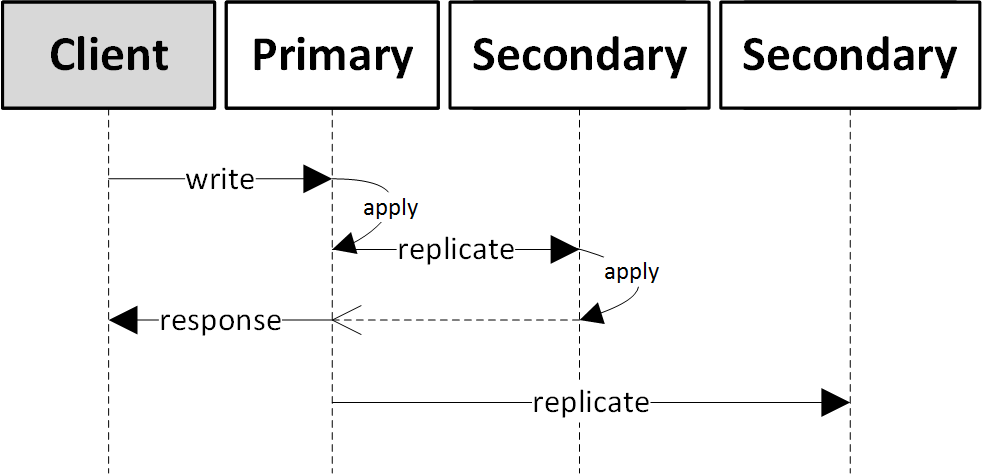
\includegraphics[width=\linewidth,keepaspectratio]{images/write-concern.png}
\caption{Write process with write concerns}
\label{write-concerns}
\end{figure}
\textit{Read preferences} allow the administrator to route read operations. They determine from which node a client is allowed to read. MongoDB supports five read preferences:
\begin{itemize}
  \item \textbf{primary:} all read operations are requested to the primary node
  \item \textbf{primaryPreferred:} read operations are requested to secondaries, if the primary is unavailable
  \item \textbf{secondary:} read operations are requested to secondaries
  \item \textbf{secondaryPreferred:} read operation are just requested to primary, if no secondary is available
  \item \textbf{nearest:} read operations are requested to the node with the lowest network latency
\end{itemize}
\cite{mdbdocu}
\subsection{Sharding}\label{mdb-sharding}
If the amount of data exceeds the capacity of a single database server, partitioning is needed to distribute the data on multiple servers. For MongoDB this ability is even more important, because it uses memory mapped file I/O to access its underlining data storage \cite{Hows2013}. MongoDB uses a horizontal partitioning mechanism called \textit{sharding}.\\
The data collection gets divided and distributed onto multiple servers called shards. Every shard is an independent database managed by multiple \textit{mongod} processes. All the shards are combined to one logical database. The partitioning and routing are managed by the earlier mentioned \textit{mongos} (\ref{mdb-core}) process. All write and read requests of an application are send to a \textit{mongos} process, that holds the information where the requested data is stored and forwards the requests to the responsible \textit{mongod} processes. The data is distributed based on a configured \textit{shard key} and chunk size. The metadata of a sharded cluster is stored on special config servers, where the \textit{mongos} processes can obtain the routing information \cite{Edward2015,Hows2013}.

\subsection{Summary}
Figure \ref{arch-example} describes one possible deployment architecture, that contains all in this section mentioned artifacts. Clients can connect to a \textit{mongos} process, running on an application server. This process forwards the requests, based on the information stored on the \textit{config servers}, to the right shard. A shard is an replica set, containing several \textit{mongod} processes. The \textit{shard key} in this example is the year. So Shard-1 contains all data from 1999 til 2009 and Shard-2 contains the data from 2009 til now. 
\begin{figure}[H]
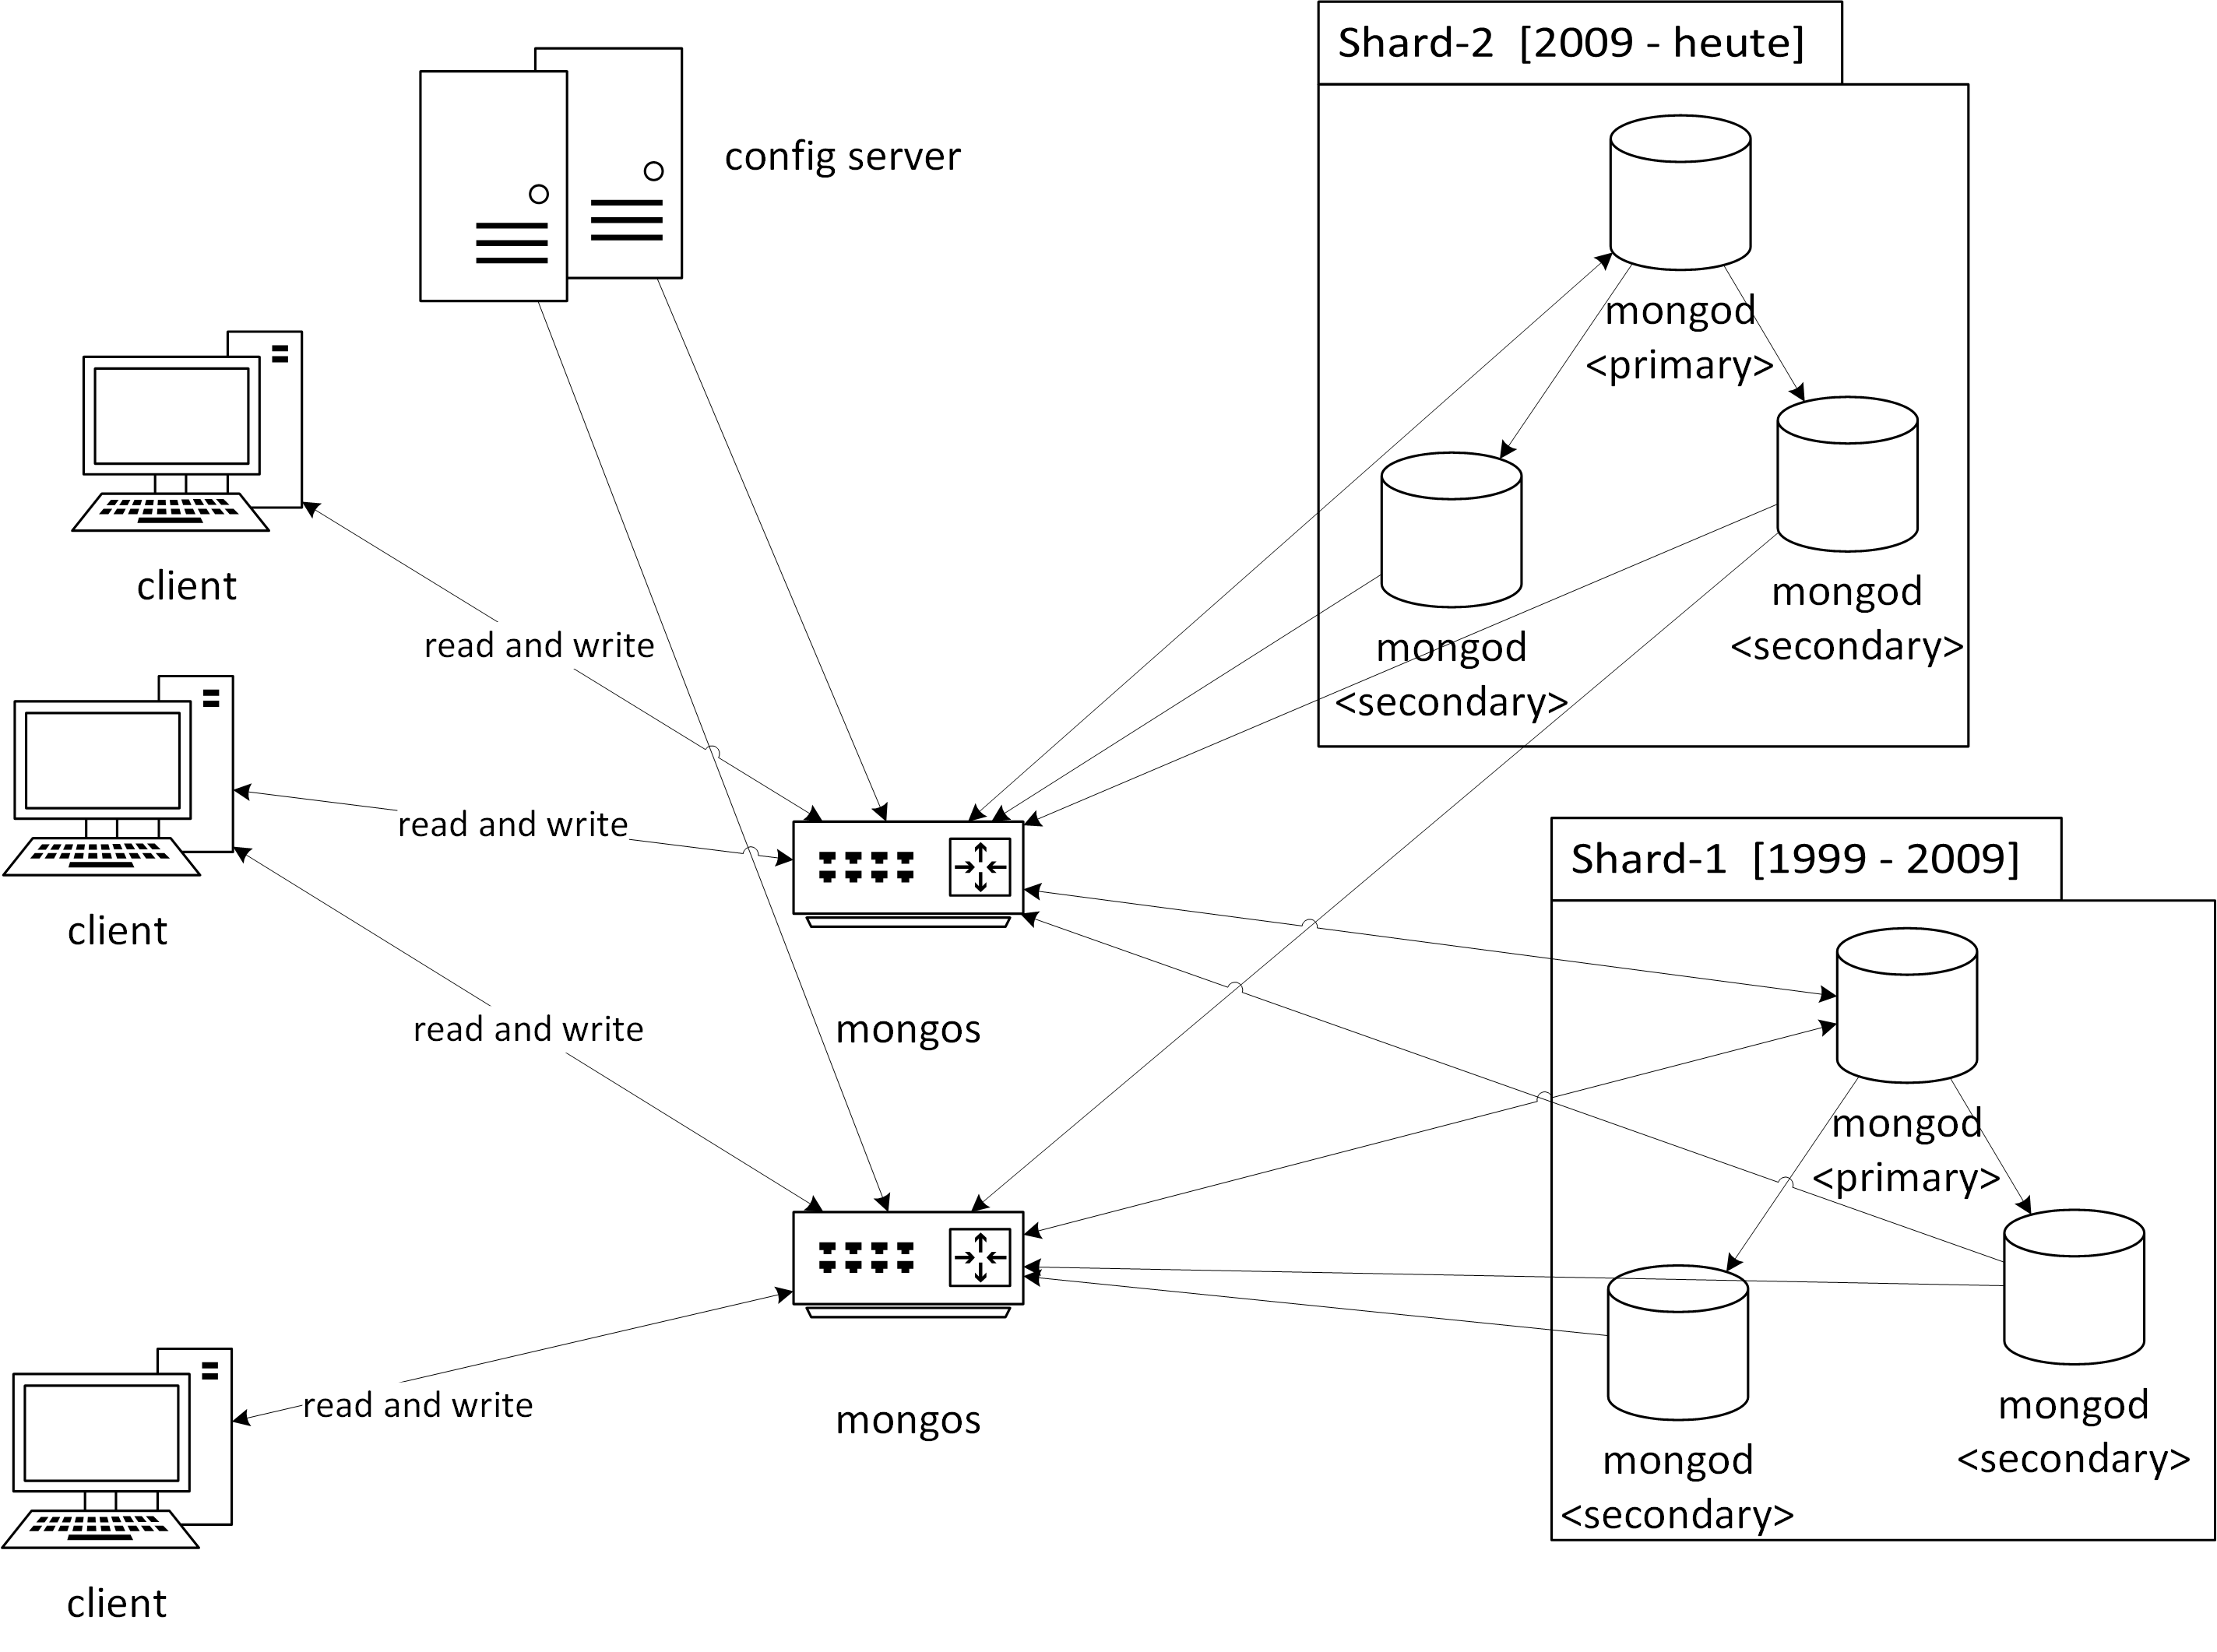
\includegraphics[width=\linewidth,keepaspectratio]{images/sharding.png}
\caption{MongoDB Architecture Example}
\label{arch-example}
\end{figure}

\section{Performance}
\subsection{Performance measurement introduction}
Before a performance measurement or comparison between database systems can be made, it is necessary to define the performance indicators. Depending on the use-case of the measured databases the results can be completely different. For example a real-time system is a lot more dependent on access times, latency and fast updates for concurrent users. A scientific database has to be fast at processing complex queries with joints and preprocessing routines like aggregation \cite{Neil_O}. Of course the benchmark should be implemented to test the performance of a database system in a way that reflects your usage in the future.
\\\\
For database systems there is a council called the TPC . This organization tests different database systems on physical and virtual machines and scores them by performance. The performance indicators can be seen on their website and there are different benchmarks depending on the use-case of the system \cite{_tpc.org.}. 
\\\\
Another standardized benchmark for database implementations is the Wisconsin Benchmark. This was one of the first standardized benchmarks and was made for relational databases. The test contains of inserts, selections, joints and projections. For further details on this benchmark, see the paper \cite{DeWitt_The_1991}.
\\\\
This paper will summarize MonogDB performance compared to other popular NoSQL and SQL  databases.

\subsection{Influencing factors to database performance}
All the results provided by this paper are dependent on the underlying hardware used. Depending on the host system for the database application, the performance can vary a lot \cite{Lee_W._2009}. Examples for big performance factors are available memory, processor speed and the used storage.
\\\\
For evaluation which database system should be used, it is important to know on what kind of hardware the production system will run. This is due to the fact, that different database systems were developed to meet certain performance goals on different hardware. Therefore some databases scale well with more memory and memory bandwidth since they try to cache a lot of the data in system memory. But there are also databases which try to be very lightweight on memory for low end systems or massive I/O  operations \cite{Boncz_Database_1999}.
\\\\
Nearly all databases are reliant on the used storage. This storage is the only way to keep the data, even when the system is turned off. Even In-memory databases use the persistent storage to save their current data \cite{Wang_Main_2001}. As transactions ultimately have to be written to the storage, this becomes the biggest bottleneck. With traditional HDDs having a high latency when accessing random data, which happens frequently on a database system, the introduction of SSDs  eliminated those problems. Benchmarks done on traditional HDD storage can be translated most of the time to SSDs since all databases will perform better but should stay at the same relative performance.
\subsection{NOSQL compared to SQL databases}
It is often one of the first question, when talking about database performance. SQL or NOSQL, which one is faster? Comparing those two types of databases generally, is not really useful. The way how data is stored is completely different and the use-case defines if SQL or NOSQL fits better.
\\\\
A good example for the difference of these two types is Twitter. They use a NOSQL database for all the tweets. Although Twitter is using MySQL heavily. The reason for this is easy to explain. A tweet contains some sort of content like text or images and a lot of additional information like hashtags, user and topics. Storing that data in a relational, normalized way, it would take a lot of tables and joins to represent a tweet . All hashtags would be referenced over multiple tables. These joins take time and since Twitter is a real time platform, latency should be low \cite{Weil_21}.
\\\\
In contrast the NOSQL implementation is way easier. The complete Tweet is stored as a document. The hashtags and links are stored in the same document in a key value manner. Now when you want to read 100 Tweets, in a NOSQL context, this can be done by one simple query. In a relational model, complex joins for each Tweet would be necessary. In such a scenario performance is obviously on the NOSQL side, but only because the use-case is well suited for non-relational models.
\subsection{MongoDB performance}
This paper will be limited to benchmarks of low level functions for databases. These functions are: reads, writes and deletions. Performance is measured between MongoDB and MariaDB. MariaDB is a SQL database and as previously mentioned, general comparisons between NOSQL and SQL are not useful. In this case two implementations of SQL and NOSQL are compared which is relevant when the use-case can be implemented by both designs without drawbacks. In such a scenario, raw performance is a valid factor.
In addition to the benchmark implemented by the author of this section, another one is used for validity and a broader overview. The referenced paper contains additional databases.
\\\\
The following performance test were performed, using NodeJS. For MongoDB connectivity the official MongoDB driver  was used. The same applies for the MariaDB driver . The driver selection can cause huge performance differences. There are several MariaDB drivers for NodeJS and of course other programming languages. Therefore comparisons of database performance should be done, using the same programming language \cite{_mscdex.}. The inserted data contains just an id represented by an integer.
\begin{figure}[H]
\includegraphics[width=\linewidth,keepaspectratio]{images/Performance_Inserts.JPG}
\caption{Insert MongoDB vs MariaDB}
\end{figure}
\begin{figure}[H]
\includegraphics[width=\linewidth,keepaspectratio]{images/Performance_Deletion.JPG}
\caption{Deletion performance}
\label{arch-example4}
\end{figure}

The numbers show an interesting result. In the insert test MongoDB performs worse than MariaDB just slightly up to the point of 1000 inserts. After that point MariaDB falls behind. With increasing number of inserts the performance leap of MongoDB increases a lot. A reason for this could be some kind of overhead for inserts on MongoDB, further investigation is needed to evaluate the results and the cause. A similar behavior can be seen on deletion test.
\\\\
The following performance results are provided by the paper \cite{Li_A_2013}
\begin{figure}[H]
\includegraphics[width=\linewidth,keepaspectratio]{images/Performance_Reads.JPG}
\caption{Time for read operations in milliseconds}
\label{arch-example2}
\end{figure}
\begin{figure}[H]
\includegraphics[width=\linewidth,keepaspectratio]{images/Performance_Writes.JPG}
\caption{Time for write operation in milliseconds}
\label{arch-example3}
\end{figure}
\begin{figure}[H]
\includegraphics[width=\linewidth,keepaspectratio]{images/Performance_Delete.JPG}
\caption{Time for delete operation in milliseconds}
\label{arch-exampl1}
\end{figure}

Interestingly the benchmarks from the paper show similar results on write performance when comparing the SQL implementation and MongoDB. After 100 writes MongoDB performs better. When comparing to other NoSQL databases, MongoDB is always in the upper half of the field. So it can be said, that this database should be suited well for demanding applications and performance shouldn't be a major problem. 
\\\\
These statements only apply for single instance usage. Since MongoDB uses a single master architecture for multiple instances, throughput will be less than database systems that trade consistency for performance. Using sharded servers can increase performance for horizontal scaling. With this addition, MonngoDB is also very usable for scientific applications with high amounts of I/O and data \cite{Dede_Performance_2013}.




\section{MongoDB and Big Data}
In terms of Mobile Applications, IoT, Industry 4.0 and cloud-computing, data is vast, unstructured, sometimes unwieldy and complicated. In this context, Big Data is identified by its velocity, variety and volume. Therefore, requirement and expectations has changed how to store, process and analyze data. It has led to the development of NoSQL databases such as MongoDB\cite{MongoDBInc.2013}.
\\
However, in the era of Big Data, there a 2 kind of database solutions for facing Big Data. We distinguish operational Big Data Systems and analytical Big Data solutions. Features of Operational Big Data Systems provides real-time, interactive, dynamic workloads that ingest and store data. MongoDB belongs to this category and is a popular technology for operational Big Data applications\cite{MongoDBInc.2013}.
\\
On the other hand, Analytical Big Data technologies are useful for retrospective, sophisticated analytics of your data. A most-known example of an Analytical Big Data technology is Apache Hadoop. Hadoop is designed for storing and processing large sets of data on a distributed environment based on commodity servers and storage. It is an open-source Apache project, which consists of a distributed file system called HDFS (Hadoop Distributed File System) and a data processing and execution model called MapReduce\cite{Wadkar2014}.
\\
Choosing between operational and analytical Big Data solution isn’t the right way of thinking about facing this Decision. Many organizations are harnessing the power of Hadoop and MongoDB together to create complete big data applications. At the one hand, MongoDB powers the online, real time operational application, serving business processes and end-users, exposing analytics models created by Hadoop to operational processes. At the other hand, Hadoop consumes data from MongoDB, blending it with data from other sources to generate sophisticated analytics and machine learning models. Results are loaded back to MongoDB to serve smarter and contextually-aware operational processes – i.e., delivering more relevant offers, faster identification of fraud, better prediction of failure rates from manufacturing processes\cite{MongoDBInc.2013}.
\\
In the following, you see a Figure which shows a Design pattern how to combine these two technologies to be ready for a Big Data environment:
\begin{figure}[H]
\includegraphics[width=\linewidth,keepaspectratio]{images/bigdata.png}
\caption{Design pattern for integrating MongoDB with Data Lake~\protect\cite{MongoDB2016}}
\end{figure}

\section{Conclusion}
All in all, MongoDB is a powerful and popular documented-oriented database. It comes with a lot of features, which meets the modern-day requirements and challenges for business applications, platforms and the web. 
The examples about the MongoDB data model, queries and CRUD operations showed how easy it is for developers to setup and work with this database. MongoDB is also very flexible in terms of extending the structure of documents. However, it is strongly recommended to consider the usage of common patterns to create a strong and future-proof data model. The usage of patterns will also help developers to understand a given database structure and work together on larger projects.
Even in a big data context MongoDB is a good choice for big data applications. That is why you will find a lot of companies and startups using MongoDB in their development.

\subsection{MongoDB in CAP-Theorem}
In a single server or Master/Slave configuration MongoDB prioritize consistency over availability. That might be the reason why in most literature MongoDB is positioned at CP-side of the CAP-Theorem. But in \textit{Replica Sets} it is possible to trade some of the consistency for a higher availability, by configuring \textit{read preferences} (\ref{read-write}). By allow reading from secondaries, there is no way to ensure the client is reading consistent data. \anfuc{This behavior is characterized as eventual consistency, witch means that although the secondary's state is not consistent with the primary node state, it will become consistent over time}{p. 108}{Edward2015}. With \textit{write concerns} (\ref{read-write}) it is possible to obviate inconsistent reads happen to often, by ensure that a minimum number of secondaries is consistent. \\
Figure \ref{mongodb-cap} describes how the three values change depending on the configuration. The partition tolerance is always fulfilled, because MongoDBs architecture is designed that way. By allow reading from secondaries availability will be increased at the expense of consistency and some consistency can be recovered using \textit{write concerns}. But availability is always limited to reading, so it can never be fulfilled for all aspects of an application.
\begin{figure}[H]
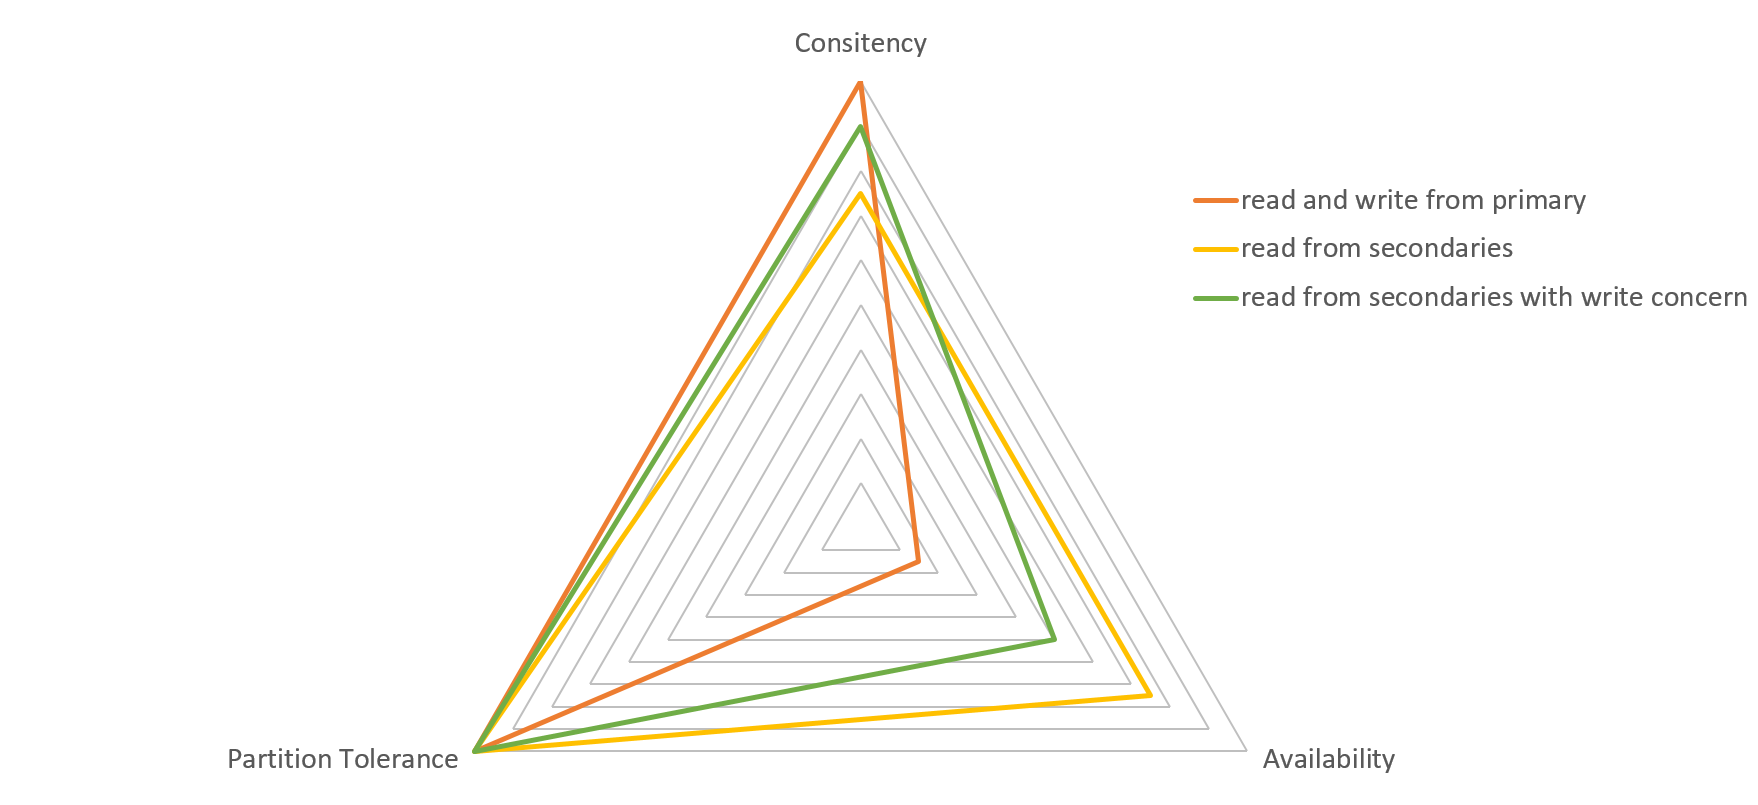
\includegraphics[width=\linewidth,keepaspectratio]{images/mongodb-cap.png}
\caption{Write process with write concerns}
\label{mongodb-cap}
\end{figure}

\chapter{RethinkDB}
\section{RethinkDB}

This chapter briefly introduces the major topics around RethinkDB, a real time open source shema-less document-based database. It is widely used by startups and Fortune 500 firms such as NASA, GM and Distractify. Founded in 2009 RethinkDB saw major funding by Y Combinator, had their first release 2012 and went to version 2.0 in 2015. October 2016 the company behind RethinkDB closed down due to the lack of business success but the software got then purchased in February 2017 by a Linux Foundation daughter: The Cloud Native Computing Foundation. It has then been re-licenced under Apache Licence 2.0, going away from their initial copyleft-like licence \cite{RethinkCNCF,techcrunchredb}.   

\section{How RethinkDB works}

\subsection{Data storage in Rethinkdb}

\subsubsection{The data structure}

RethinkDB stores data as a B-tree-structure. A B-tree is a data structure which is balancing itself and allows filtering and sorting within logarithmic time. This B-tree is saved on a file system instead of the RAM in large structures \cite{BTreeTechTarget}. This file system is called BTRFS (B-Tree File System),  This enables the copy-on-write scheme provided by BTRFS thus making it possible to repair saved data from the copied clone. Other benefits to this filesystem are a garbage compactor to reduce older copies, low cpu-overhead, optimization for solid-state drives, data consistency (more detail about consistency in the ACID and CAP chapter \ref{acidcap} , b-tree aware caching and multi version control\ref{mvcc}. B-Tree aware caching is a way to give RethinkDB the capability of using far more data than available RAM.\\
RethinkDB does not include a hardware data consistency, this has to be maintained by the used file system itself, which RethinkDB supports the most commonly available \cite{RethinkDataStorage}


\subsubsection{partioning and multi-datacenter support}

Data in RethinkDB can be saved on multiple servers. This is done by replicating databases and providing each of them with a specific tag such as 'de\_east' or 'westeros'. A table can have an non-specific amount of replicas on each server. 
On servers data can be partitioned into shards and furthermore tagged like replicas.  The partition is done by a range of specific sharding algorithms and uses the primary key of each table. This means, that a shard key and a primary key is identical. For example if a data set has a primary key containing only letters and is ordered alphabetical, the sharding algorithm will likely split the data around the key 'm'. Thus the new two partitions containing every data with a key from 'a' to 'm' and from 'n' to 'z'. Evidently this algorithm always tries to part at the best pivot to have new partitions in equal size.\cite["How does multidata-center support work"]{RethinkSharding}

\subsection{The atomicity model}
\label{atomicity}
Atomicity means, that either the complete stack of operations will be executed or non at all, there is no middle ground \cite{TechTargetAcid}.
Operations within single json documents are guaranteed to be atomic, queries accessing different keys are not as they may be inconsistent in read and write operations \cite{jepsen2016}.
The atomicity differs itself from other NoSQL databases by the way, that every set of operations, every chained query is atomic by the restriction named above. Plus, another limit is, that upon executing a non deterministic operation RethinkDB will nolonger be able to ensure their atomicity. In this case, RethinkDB will automatically throw an error by default. This behaviour may be shut by setting the according flag \cite["How does atomicity work"]{RethinkQE}.  

\subsection{ACID and CAP theorems in RethinkDB}
\label{acidcap}
RethinkDB’s architecture is based, as mentioned in the section above \ref{atomicity}, on the atomicity model. This model is part of the ACID paradigm for databases. ACID is a acronym for atomicity, consistency, isolation, and durability and describes the key desired parameters during a transaction to and off of a Database. ACID is norminized under ISO/IEC 10026-1:1992 Section 4 \cite{TechTargetAcid}. 
RethinkDB has also support for every other ACID paradigm except full isolation and absolute data consistency and therefore might not the best choice if full ACID-Support is needed. But RethinkDB provides a basic consistency as specified within the CAP-theorem. What this theorem is, has been elaborated within the Architectural Basics of Cassandra \ref{captheroem}. The basic consistency within RethinkDB has been ensured by the fact, that every shard has a single replication and read and write actions are performed on this replication but not on the shard itself. Data remains immediately consistent and conflict-free. 
The Database also provides availability needed by the CAP-theorem as data is also accessible both up-to-date and out-of-date. Out-of-date queries are executed on a snapshot and without trying to get the most current data set. This means, that these queries are faster and guarantee availability but may not return nor access the most current data. The up-to-date queries are assuring that they return the latest data consistent and artifact-free. As before mentioned data is not absolutely consistent. This tradeoff roots within the partitioning. RethinkDB assures data to be consistent on the same network but cannot do the same for network partitions if data has to be up-to-date.\cite{RethinkCAP}. 

\begin{figure}[H]
	\begin{center}
		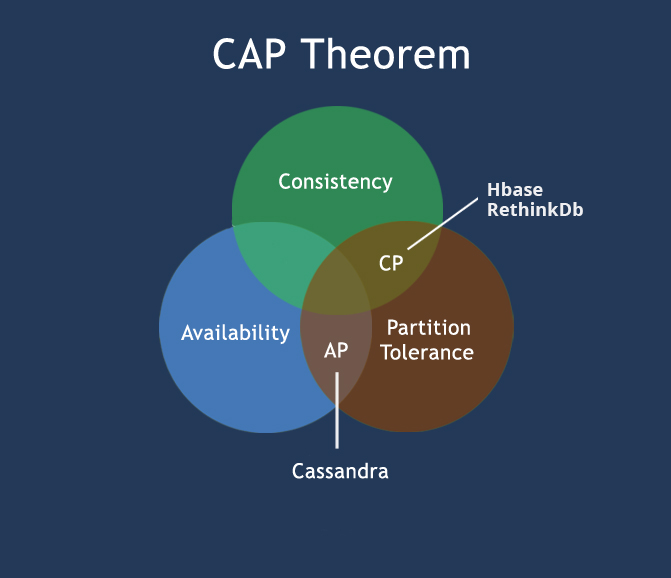
\includegraphics[scale=0.6,keepaspectratio]{images/captheoremnosql.jpg}
		\caption{Position of RethinkDB in the CAP-Theorem \protect\cite{rdbcaptheorem}}
	\end{center}
\end{figure}

\subsection{multiversion concurrency control}
\label{mvcc}

RethinkDB has built-in support for multi version concurrency control. This means, that every writing operation is by default only made after a snapshot, simply a read operation, has been taken off of that tree. This has following benefits:
\begin{itemize}
	\item Easy roll backing to previous data
	\item Lock-Free read and write operations
	\item Enables non-blocking queries making real-time hour long possible
\end{itemize}
\cite["How are concurrent queries handled?
"]{RethinkQE}

\section{The query language ReQL}

RethinkDB has its own query language called ReQL. A query contains the table, an action and the order to run on a specific database connection. For Example the query to get an id (1) from a table (test) looks like this:

\begin{lstlisting}[frame=single, caption=get document from Database  (javascript driver), label=rget]
r.table("test").get(1).run(connection)
\end{lstlisting}

One idiomatic aspect of ReQL is already evident in this example. ReQL is a chain of commands. Multiple queries can be written as a one-liner and are thus executed as one without disturbance. If there are dependencies on another query one should use this chain-technique to make sure it is executed in the right order. This works due to the fact, that the query is only parsed and executed on the server while being build on the client. On top of that, RethinkDB is lazy executing the queries.  It immediately stops upon satisfaction. 
Furthermore are those queries functional and allows adding lambda functions as parameter. RethinkDB has build-in support for example for javascript code through the V8-Engine, map-reduce, table-joins and math \cite{reql}.

\begin{lstlisting}[frame=single, caption=create the table 'test', label=createTable]
r.db("test").tableCreate("test", options).run(connection)
\end{lstlisting}

Every table created gets a primary key for indexing. By default it is id but this can be changed by providing an option:
\begin{lstlisting}[frame=single, caption=options for create table, label=cTableOptions]
{primaryKey: 'name'}
\end{lstlisting}

By setting this option as in the example, the table now is indexing every row under „name“.
TableCreate has, as most of the  many different options available, accessible in their documentation \cite{tableCreate}. 

\subsection{query executing}

RethinkDB has a special way of executing a query. One key point is, that the query is not executed on a client but on the server itself. By receiving the query, the server creates a list of instructions consisting of internal logical operations. RethinkDB now tries to make this list as efficient as possible by executing most basic operations first and more time consuming, such as manipulating data last. Each operation set is called Node and their complexity ranges from single document queries to deep complex subquery commands. After executing, the server returns his result as a datastream not only to the client itself but also to every other relevant server. This has the benefit, that RethinkDB does not really care on which server the query is executed and therefor can parallize this process.
\cite["How does RethinkDB execute queries?"]{RethinkQE}

\section{RethinkDB perfomance analysis}

RethinkDB had has a major performance issue since its start but kept on improving on this aspect over the years. For example in a comparison in 2014, MongoDB has been 3 times faster than RethinkDB at executing queries over a large patent data set\cite{rvsm2014}.
A newer comparison of 2015 turns this around but only for writing data to the database. Reading, RethinkDB has still been half as fast as MongoDB has been in that benchmark\cite{rvsm2016}.
Within an official benchmark test, the RethinkDB Team got this result:

\begin{figure}[H]
	\begin{center}
		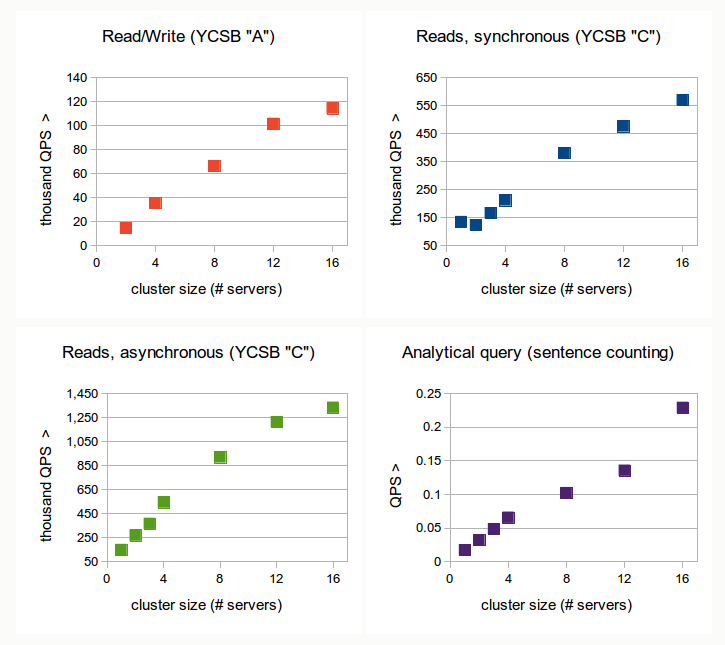
\includegraphics[scale=0.6,keepaspectratio]{images/performanceReport.png}
		\caption{Performance Report of RethinkDB \protect\cite{performanceReport}}
	\end{center}
\end{figure}

They states, that in their working environment they were able to perform around 16 000 queries in a second (QPS). For this benchmark, RethinkDB used "analytic workloads in a simplistic but very common fashion" \cite{performanceReport}.
\section{Limits}

As every existing technique RethinkDB, too, has restictions. 
These can be hard or soft limitations depending on their context.
\cite{RethinkLimits}

It is not possible to create more than 64 Shards in RethinkDB.
The number of databases are not limited by anything than diskspace and RAM as is the number of tables.
The recommended size limit for a single Document is 16MB and should be respected due to potential perforance issues.
Also do Arrays in a RethinkDB Server have a limited length.
This length can be configured per query and by default is at 100.000 elements.
Primary keys are limited to 127 characters.
But secondary keys aren't hard limited by those 127 characters, if they exceeds their limit, RethinkDB will use linear search for the following characters.

JSON queries are hard limited as well.
They can only be 64 MB in size or smaller.

The ordering in RethinkDB is byte-wise.
The functions orderBy and between uses the byte representaiton of the carater.
This has the result that RethinkDB dose not normalize identical characters with multiple codepoints.
For example the character "é" has the UTF-8 representation \code{\textbackslash{}u0065\textbackslash{}u0301} and \code{\textbackslash{}u00e9}, the will be grouped separately.

The usage of the cli option \code{--direct-io} is restricted to supporting file systems only.
Typically encrypted and compressed file systems will not support this option.

Numbers are double precision IEEE 754 floating point.
Integers are stored precisely from -2\textsuperscript{53} to 2\textsuperscript{53}, outside that range they will be rounded.

\section{Data Types}

RetinkDB has all the basic Data types. 
Number, string, boolean, object, array and the \code{null} value. 
Additionaly RethinkDB stores specific data types like tables, streams, selections, binary objects, time objects, geometry data types, and grouped data.
\cite{RethinkDataTypes}

\textbf{Numbers} can bee Integer or Floatingpoint values. 
They will be stored with 64-bit percision.
\code{NaN} or Infinit can not be stored.

\textbf{String} are stored with UTF-8 encoding.

\textbf{Booleans} can be \code{true} or \code{false}

\textbf{Null} is a special value.
It is not the number zero or an empty string.
It symbolizes the absence of any other value.

\textbf{Objects} are key-value pairs.
Any valid JSON object is a valid RethinkDB object.
\begin{lstlisting}[frame=single, caption=RethinkDB's object notation, label=refdoc]
{
	"key"  : "valueString",
	"key2" : false,
}
\end{lstlisting}
The keys can only be strings, but the values can be any data type.
A RethinkDB Document is a object.

\textbf{Arrays} are lists of values.
Arrays can be empty.
It is not enforced to use only on type of values in an Array.
But it is highly recommended.
\begin{lstlisting}[frame=single, caption=RethinkDB's array notation, label=refdoc]
[
	"valueString",
	false,
]
[]
\end{lstlisting}
The values of an Array can be any data type.
If you use arrays for many values, more than 100.000 you should notice that arrays are fully loaded into Server RAM before being send to the client.

Specific Data types

\textbf{Databases} are returned after a \code{db} function call.

\textbf{Tables} are returned after a \code{getAll} function call.
Their behavior is similar to selections.

\textbf{Selections} are the result of \code{filter} ot \code{get} function calls.
Selections comes in three variants \code{Selection<Object>}, \code{Selection<Array>} and \code{Selection<Stream>}.

\textbf{Streams} are like arrays, lists.
Streams are not writable and are lazy, they give you the next dataset if the current has been processed.
With Streams you can read tremendous long lists of Data, without holding everything in Memory.


\section{Changefeeds}

Changefeeds are the main part of RethinkDB's real-time functionality.
Almost all queries can be used as a changefeed.
With a Changefeed you recive any changes on your query.
\cite{RethinkChangefeeds}

\begin{lstlisting}[frame=single, caption=implementing changefeed, label=refdoc]
r.table('project').changes().run(conn, (err, cursor) => {
	cursor.each((err, row) => {
		if(err) throw err;
		processRow(row);
	})
});
\end{lstlisting}

The \code{changes()} method returns a cursor.
The \code{each()} method of that cursor object iterates over each change.
If the underlaying data of the query changes the callback of \code{each()} will be called.
For example a new project will be added \code{{id:3, name: "awesome Project", priority:1}} into the project table.
The \code{each()} callback will be called with the changes of the table.

\begin{lstlisting}[frame=single, caption=changefeed's return value, label=refdoc]
{
	old_val: null,
	new_val: {id:3, name: 'awesome Project', priority:1}
}
\end{lstlisting}

If the callback for \code{each} returns false, the cursor will stop iterating.

\textbf{single document changefeeds}

The single document changefeed only notifies the subscriber if the document changes.

\begin{lstlisting}[frame=single, caption=single document changes, label=refdoc]
r.table('project').get(3).changes().run(conn, callback);
\end{lstlisting}

This would listen for changes of the project with id 3.

\textbf{Filtering Changefeeds}

The method \code{changes()} integrates with the ReQL language.
\code{changes()} can be used with mostly any outher command.

The chaning of ReQL methods can be as complex as you wish.
For Example changefeeds can be filter:

\begin{lstlisting}[frame=single, caption=filtering changefeeds, label=refdoc]
r.table('project').changes().filter(
    r.row('new_val')('priority').lt(r.row('old_val')('priority'))
)('new_val').run(conn, callback)
\end{lstlisting}

This will be notified on every change, there the priority is lower as the previous.
Chaining methods with changefeeds has some limitations.


\textbf{handling latency}

With some latency on the client side, it is possible that there will be mutliple writes into a table, before the clinet gets all changefeed events.
By default a changefeed subscriber will only get one change object.
If this is not the desired procedure the option \code{squash: false} should be used on the \code{changes()} method.
With this the change object will be send for every change.

Changefeeds do not have a delivery guarantee.


\section{Conclusion}

RethinkDB is a highly potential database with many use cases and some valuable customers. Being consolidated under the Linux Foundation, this potential might be more furthered and current problems, like the performance issues reduced. In this future, the lack of documented community drivers will hopefully evaporate and more and more third libaries will be added to RethinkDB.  Even though the namespacing, with just the \textit{r}, might be strange to use at first but due to the query chainability, it's many functions and the changefeed make up a lot for the uncertainty resulted in shut down and revival. RethinkDB's easiness in usability and installation-wise, it's simple web interface and the well-elaborated documentation are reason enough to give it a shot.

To synthesize it, RethinkDB is worth considering for web \& app projects alike especially if real time support is needed.

\part{Graphbased DB}
\chapter{neo4j}
\section{Introduction to Graph Databases}

Nowadays a huge number of different databases systems exist. You always must select the best suiting one for your specific use case. Data is often ordered in relations between objects, like different cities and their connecting streets. 
If there is the possibility to structure your data in the database the same way as the data is structured in real life, you may get a speed and usability advantage out of that. The best solution to picture these structures is to use the graph. That is why graph databases have been developed, which now will be presented to you.

\subsection{Graph Databases}

Graph databases use graph structure to order data in the database. There is more than one solution for using graphs. The main aspects of the first are nodes and edges, which are essential for the database structure \cite[pp. 1-4]{RobinsonWebberEifrem.2013}.
The connection between the nodes are the relations of the data. In the example picture below \cite[para. 1]{Rouse.2016}, you can see how graph databases work with the nodes and their relations. For example you can see the married couple Julie and Bob.

\begin{figure}[H]
	\begin{center}
		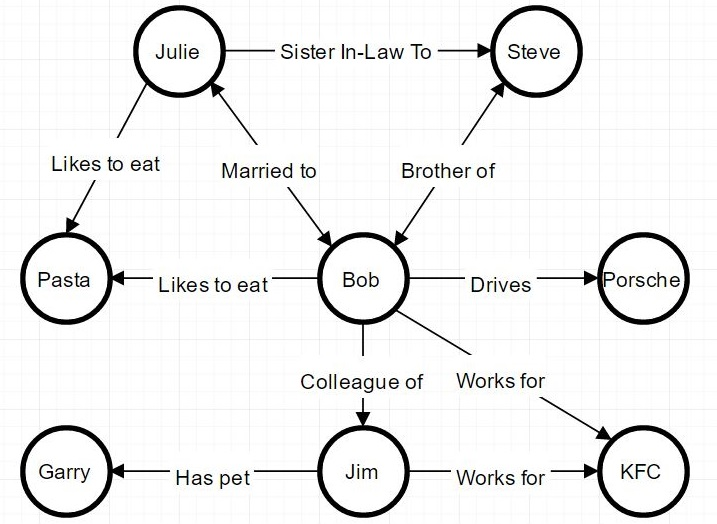
\includegraphics[scale=0.8,keepaspectratio]{images/neo4j/IntroExampleGraph.JPG}
		\caption{ExampleGraph}
	\end{center}
\end{figure}

You can also build property graphs, which you can use for routing. For example, you can find the shortest way from one city to another. The special thing about property graphs is, that attributes can be added to the nodes and edges. So you can store further information in your graph \cite[p.3]{RodriguezNeubauer.2010}.

The second one is used for the semantic web and concentrates on triples. Semantic web stands for machine processable web. In the semantic web the W3C consortium defined a framework how to work with the triples \cite["Overview", para. 1]{W3C.2014}. It is called Resource Description Framework and its structure is like following:

\begin{itemize}
	\item First part: subject, where the relation starts.
	\item The second: predicate, the relation
	\item The third: object, where the predicate points to.
\end{itemize}  

Despite you can see the same node and edge structure, it is different to the property graphs. In Resource Description Framework, which is the most common used framework, you can only build connections between the nodes, but you can neither set properties to the nodes nor to the edges.

\subsection{Neo4j}

Neo4j - developed by Neo Technology - is one of the first and up to now the most popular graph database implementation. Neo4j is more than five times popular than the second graph database - OrientDB  \cite[para. 1]{SolidITGmbH.2017}.\\
Its first Version was released in 2010 after three years of development. It is called as transactional, disk based database, which follows the ACID principle \cite["Neo4j Internals", para. 4]{NeoTechnologyInc.2017b}. The implementation is in Java and can be used in two different license models. The Community and the Enterprise Edition.\\
The Community Edition is free, but only running on a single node. You can use all the features of Neo4j without high availability through clustering and hot backup. 
These additional modules are coming with the Enterprise Edition only. There are some further categorizations for the Enterprise version like the test licenses Evaluation, the Educational and the Neo4j Loves Open Source licenses \cite["About Neo4j Licenses", para. 1]{NeoTechnologyInc.2017a}.\\
Neo4j uses Cypher as query language. With indexing and the labels of the graph it helps to accelerate the queries, which is one of the main advantage of using graph databases and especially Neo4j.

Now you get a deeper insight into Neo4j and its data structure.

\section{Data Structures}

In opposite to the bulk of NoSQL databases Neo4j as a graph database is focused on the relationships between data.
Therefore the data structure is based on two components: nodes and relationships. Both of them can contain a variety of informations.
Let's start with the nodes. Each node consists of a JSON object which defines its properties, so the nodes can be compared to documents in MongoDB for example. In the definition of this node properties you can use anything, that's provided by the JSON standard. In a library for example we could have books with properties about their title, page number or publication date.
With this properties we get the ability to store data and in connection with the later introduced cypher query language we can search for nodes by them. But currently searches would be executed over the whole graph and any node can contain different properties.
\cite["Nodes", para. 3]{NeoTechnologyInc.2017c} \cite[p. 80]{Gupta.2015} \cite[slide 20-21]{Hunger.2013}

\begin{figure}[H]
	\begin{center}
		\includegraphics[keepaspectratio]{images/neo4j/data-structure/single-node.png}
		\caption{Single Book Node}
	\end{center}
\end{figure}

To structure the data, every node can be labeled. This labels can be interpreted as  a typing. Looking back at our library example we could create nodes labeled as “book”, “author” or “borrower”. By labeling the node we organize them in sets, like the MongoDB collections or SQL tables.
Beside the better structure we achieve a more efficient searching, because the amount of data to search in can be reduced right at the beginning, by the definition of the node set (label) to search in.
At this point we have nodes with properties organized in sets by their labels, but no relationships.
\cite["Labels", para. 2]{NeoTechnologyInc.2017c} \cite[slide 26-27]{Hunger.2013}

\begin{figure}[H]
	\begin{center}
			\includegraphics[keepaspectratio]{images/neo4j/data-structure/labeled-nodes.png}
			\caption{Labeled Node Sets}
	\end{center}
\end{figure}

The relationships in Neo4j are quite similar to the nodes. They are also able to take properties in form of JSON objects and has labels to define their type or in this case better to say their function. In the library example a relationship between book and borrower could be labeled as “borrowed” and contains properties like “borrowDate”, “returnDate” or maybe “rating”. Here we should also have a look at a good structure, so it would be better to extract the rating and put it in another relationship like “read”.
The main and obvious difference are the two connected nodes. So every relationship needs exactly two nodes connected to it. But they do not have to be different, so it'’'s possible to point a relationship on its own origin. Naturally the node labels are irrelevant here, so relationships can be defined inside and between node sets.
\cite["Relationships", para. 1]{NeoTechnologyInc.2017c} \cite[p. 81-82]{Gupta.2015} \cite[slide 22-25]{Hunger.2013}

\begin{figure}[H]
	\includegraphics[width=\linewidth,keepaspectratio]{images/neo4j/data-structure/node-relationships.png}
	\caption{Related Nodes}
\end{figure}

After looking at the elements of the Neo4j data structure, we will now have a look at how we create this structure in our database instance.
At first it'’'s necessary to create some nodes. Therefore we use the CREATE command followed by round brackets to define the node itself. The first element of the node definition is an optional variable name at first to save the reference to the created node, if needed. After this a colon and label name is required to define the node set. The label doesn'’'t need to be defined before using it here. At last we enter the JSON object with our node properties and close the definition brackets.
\cite["Create a Record for Yourself", para. 1]{NeoTechnologyInc.2017d} \cite[p. 80]{Gupta.2015}

\begin{lstlisting}[frame=single, caption=Create Database, label=creategraphdb]
CREATE ( variable:LABEL {} )
CREATE ( theLordOfTheRings:Book { title: 'The Lord Of The Rings', publication_date: '1954-07-29' } )
CREATE ( jrrTolkien:Author { name: 'J. R. R. Tolkien' } )
CREATE ( johnSmith:Borrower { name: 'John Smith' } )
\end{lstlisting}

Secondly we can create the relationships. Thanks to the ascii-art syntax it'’'s easy to understand the create statements. It starts again with a CREATE and is followed by round brackets. In this case this brackets can contain a node definition again, but also a simple variable name to reference an existing node. After the brackets a hyphen connects the first node to the relationship definition part surrounded by square brackets. This definition is structured like the node definition: optional variable name, label, JSON object. An ascii arrow (“->”) connects the closing square bracket with the second node, this relation will point to. In the style of the first node we have here round brackets with a variable or a  whole node definition.
\cite["Create a Record for Yourself", para. 1]{NeoTechnologyInc.2017d} \cite[p. 81-82]{Gupta.2015}

\begin{lstlisting}[frame=single, caption=Create Relationships, label=creategraphrelationships]
CREATE (sourceNode)-[ variable:LABEL {} ]->(targetNode)
CREATE (jrrTolkien)-[ :WROTE ]->(theLordOfTheRings)
CREATE (johnSmith)-[ :BORROWED { borrowDate: '2017-03-15', returnDate: '2017-04-14' } ]->(theLordOfTheRings)
\end{lstlisting}

Below you can have a look at the created graph of the simple example.

\begin{figure}[H]
	\includegraphics[width=\linewidth,keepaspectratio]{images/neo4j/data-structure/sample-graph.png}
	\caption{Sample Graph}
\end{figure}

\section{Cypher Language}

Cypher is Neo4j's open graph query language \cite["Cypher Query Language", para. 1]{NeoTechnologyInc.2017e}. It was newly created to match the data-structures of Neo4j and to fulfill the special needs of Graph-Databases.
In addition it's based on SQL to allow an easy entry point for developers, which already had to work with SQL. \cite["About Cypher", para. 1]{NeoTechnologyInc.2017d}
Cypher's syntax provides a familiar way to match patterns of nodes and relationships in the graph.
Cypher is also a relatively simple but still very powerful language. \cite["Fazit", para. 1]{Mahler.2014}
Very complicated database queries can easily be expressed through Cypher.
This allows users to focus on their domain instead of getting lost in database access because it allows the user to state what he wants to select, insert, update or delete from his graph data without requiring him to describe exactly how to do it.

\paragraph{Example}

Cypher contains a variety of clauses. 
Among the most common are: MATCH and WHERE. \cite["A few words about Cypher", para. 3]{NeoTechnologyInc.2017f}
These functions are slightly different than in SQL.
MATCH is used for describing the structure of the pattern searched for, primarily based on relationships.
WHERE is used to add additional constraints to patterns.
For example, the below query will return all movies starting with "T", and return its cast as a collection:
\begin{lstlisting}[frame=single, caption=Cypher Example, label=cypherexample]
MATCH (actor:Person)-[:ACTED_IN]->(movie:Movie)  
WHERE movie.title STARTS WITH "T"  
RETURN movie.title AS title, collect(actor.name) AS cast  
ORDER BY title ASC LIMIT 10;
\end{lstlisting}

\paragraph{ASCII-Art and Nodes}

Cypher uses ASCII-Art to represent patterns. It surrounds nodes with parentheses which look like circles, e.g. \textbf{(node)}. \cite["Nodes", para. 1]{NeoTechnologyInc.2017d}

\begin{figure}[H]
	\includegraphics[width=\linewidth,keepaspectratio]{images/neo4j/cypher_pattern_simple.png}
	\caption{node ascii art}
\end{figure}

To reference a node at a later time, it can be stored in a variable like (p) for person or (t) for thing.
In real-world queries, there would probably be longer, more expressive variable names like (person) or (thing).
If the node is not relevant to the question, the parenthesis can also be empty ().

\paragraph{Relationships}

To fully utilize the power of graph databases complex patterns between the nodes can be expressed.
Relationships are basically an arrow \textbf{-->} between two nodes. \cite["Relationships", para. 1]{NeoTechnologyInc.2017d}
Additional information can be placed in square brackets inside of the arrow.

This can be

\begin{itemize}
	\item relationship-types like \textbf{-[:KNOWS|:LIKE]->}
	\item a variable name \textbf{-[rel:KNOWS]->} before the colon
	\item additional properties \textbf{-[{since:2010}]->}
	\item structural information for paths of variable length \textbf{-[:KNOWS\\*..4]->}
\end{itemize} 
\cite{NeoTechnologyInc.2017d} ("Relationships", para. 3)

\begin{lstlisting}[frame=single, caption=Create a Record, label=gcar]
CREATE (you:Person {name:"You"})
RETURN you
\end{lstlisting}
\textbf{CREATE} creates nodes with labels and properties.

\begin{figure}[H]
	\begin{center}
		\includegraphics[keepaspectratio]{images/neo4j/you.png}
		\caption{graph you}
	\end{center}
\end{figure}

\begin{lstlisting}[frame=single, caption=Create Relations, label=gcrl]
MATCH (you:Person {name:"You"})
FOREACH (name in ["Tobias","Kai","Manuel"] |
CREATE (you)-[:FRIEND]->(:Person {name:name}))
\end{lstlisting}
\textbf{FOREACH} allows the execution of update operations for each element of a list.

\begin{lstlisting}[frame=single, caption=Show Relations, label=gshrl]
MATCH (you {name:"You"})-[:FRIEND]->(yourFriends)
RETURN you, yourFriends
\end{lstlisting}

\begin{figure}[H]
	\begin{center}
		\includegraphics[keepaspectratio]{images/neo4j/friends.png}
		\caption{graph friends}
	\end{center}
\end{figure}

\section{Comparison with other Database Systems}

The following chapters will compare graph databases, especially Neo4j with other database systems such as relational databases and NoSQL (not only SQL) databases. In addition to plain comparisons there will also be some examples how graph databases can be used with other systems to maximmize the advantages of each system.

\subsection{Comparison with Relational Databases}

This chapter will give a basic overview of the similiarities and differences between graph databases and relational databases. More specifically this chapter will focus on Neo4j and SQL. 
In Neo4j relationships are first-class citizens. In SQL these relationships can only be created by using foreign keys and therefore Neo4j eliminates foreign keys. Each node contains a list of relationship-records. These relationship-records are organized by type and direction and can hold additional attributes. When you would normally run a JOIN-operation these records are used. This is the biggest advantage graph databases have over relational databases: The costs of expensive search and match operations are eliminated.
This leads to much higher performance levels than those of relational databases.
In addition the data models of graph databases are simpler and more expressive as seen in the below images \cite[pp. 9-10]{HungerBoydLyon.2016}.

\begin{figure}[H]
	\includegraphics[width=\linewidth,keepaspectratio]{images/neo4j/organization_relational.png}
	\caption{SQL data model}
\end{figure}

\begin{figure}[H]
	\includegraphics[width=\linewidth,keepaspectratio]{images/neo4j/organization_graph.png}
	\caption{Neo4j data model}
\end{figure}

Like SQL Neo4j also supports the transactional concepts (ACID). That means that data is never lost after it has been commited to the database.
The query language is pretty similiar, but cypher, the query language of Neo4j, is more expressive.
Following is a short comparison of the same transaction in SQL and Cypher. This example also demonstrates the strength of Cypher by eliminating two JOIN-operations. \cite["Working with Neo4j", para. 1]{NeoTechnologyInc.2017g}

\begin{lstlisting}[frame=single, caption=Cypher Statement, label=gcystm]
MATCH (p:Person)<-[:EMPLOYEE]-(d:Department)
WHERE d.name = "IT Department"
RETURN p.name
\end{lstlisting}

\begin{lstlisting}[frame=single, caption=SQL Statement, label=gsqlstm]
SELECT name FROM Person
LEFT JOIN Person_Department
ON Person.Id = Person_Department.PersonId
LEFT JOIN Department
ON Department.Id = Person_Department.DepartmentId
WHERE Department.name = "IT Department"
\end{lstlisting}

\subsection{Comparison with NoSQL Databases}

Since relationships are very important in graph databases, it's quite difficult to compare them with NoSQL databases, since they lack relations. Following statement by Webber and Robinson (2015) explains this scenario in a good way:
\begin{quotation}
	Most NoSQL databases store sets of disconnected aggregates. This makes it difficult to use them for connected data and graphs.
	One well-known strategy for adding relationships to such stores is to embed an aggregate'’'s identifier inside the field belonging to another aggregate — effectively introducing foreign keys.
	But this requires joining aggregates at the application level, which quickly becomes prohibitively expensive.
\end{quotation} \cite[p. 15]{WebberRobinson.2015}.

\subsection{Integration with other Database Systems}
This section will describe how to use Neo4j together with other database systems in a very basic way. It will not go in-depth and there will be no code examples to keep it as simple as possible.
To get the advantages of each database system, data needs to be stored in each database with its own data models. This is called polyglot programming: using multiple different languages, here multiple different database systems. There are existing tools for different database systems which can be used as some kind of connector to another system. The connectors let the other system subscribe to update events, so the data can be inserted in one database system and then added in the other system. The developers of MongoDB for example have created a tool called "mongo-connector" where other applications can listen for update events. This enables a one-way synchronization with Neo4j. Of course all the data model transformations have to be made manually, but once set up the full potential of both databases can be used. \cite["Goals", para. 1]{NeoTechnologyInc.2017h}

\section{Conclusion}

In the end you can say that Graph databases, and therefore also Neo4j, don't need joins to achieve relationships, since they are already first-class citizens. This has a huge impact on performance, since join-operations are very expensive.
As Neo4j holds its data as JSON it has a similiar structure to document based databases and could be used together. That way you can get the advantages of both systems. The only disadvantage is the need to store the whole data twice, which requires more storage.

In general Neo4j fullfills the CAP-theorem in points of \textbf{c}onsistency and \textbf{a}vailablity and doesn't provide \textbf{p}artition tolerance. Because Neo4j is relationship-oriented, trying to achieve partition tolerance can cause many side effects and complex queries would decrease the performance considerable.

Neo4j has many use cases. For example it is used by companies such as Walmart for real-time recommendations, Ebay for logistics, LinkedIn as a representation for their Social Network and TomTom for geo-routing. An interessting fact at this point was published by the Neo4j staff. They said Neo4j is not used by Facebook, which "they should" change \cite[para. 5]{Neo4jStaff.2011}.

Neo4j is mainly used for relational analytics and is hence not efficient unless you have many joins. The following chart will enforce this statement.

\begin{figure}[H]
	\includegraphics[width=\linewidth,keepaspectratio]{images/neo4j/neo4j_joins.png}
	\caption{neo4j sql comparison}
\end{figure}  
\cite[slide 19]{Dalal.2014}.

As shown in the graph, Neo4j's full potential unleashes when many join-operations are executed as the query execution time stays constantly low, whereas the execution time for inner joins in MySQL rises exponentially. Another performance aspect is, that Neo4j in its second version can automatically index often used Nodes and gets an additional speed advantage at run time.

Overall Neo4j is quite unique, but has high potential in the sector of relational databases.
It is useful to perform complex relational data queries and can be used for many different business cases.
It is still the most popular graph database and some weaknesses can be handled by using Neo4j with another NoSQL database together.


\part{Conclusion}
This work contains a comparison of several popular NoSQL databases.
The easiest way to choose a database solution on a given use case is to compare its needs to the CAP theorem.
But not every database solution fits exactly into the CAP theorem.
Each of them has its own capabilities, advantages and drawbacks.

The strenghts of column oriented databases clearly are on the fast reading and writing operations, when only accessing one single column, because not every line has to be read completely, but only the specified column.
Also, no null values have to be inserted, which saves a lot of space. Aditionally, column oriented databases are easily scalable and distributed and good for saving massive amounts of data.
The weakness is about transactions, those are handled significantly slower then e.g. on relational databases.

Key Value is an approach perfectly suited for uses cases where own keys are generated.
The main difference to other NoSQL databases is that data is only accesible over the saved key.
This aggravates the querieng of data appart from the key.
An avantage of Key Value databases is the super flexible data model.
Data sets could be saved without any type specification to a key.

Document-based nosql databases provides multiple advantages. With a single query, they are able to access huge amout of data fast. Especially compared to SQL it offers easier implementation because it stores data schema-less and enables flexibility. Over and above, document-based databases can be customized to meet certain requirements for the cap therorem like partitioning and sharding even over multiple servers through clustering. Besides to the advantages, document-based databases do have drawbacks such as the slow attribution aggregation or slow updates. In addition, all documents are stored unsorted and are completly loaded into the ram. Data is stored denormalized which causes high memory usage.

Graph databases like Neo4j take the opportunity to manage tightly related data, such as social networks or real-time recommendations. The similarity in the data structure to document based databases keeps the freedom in schema and the possibility to integrate and sync Neo4j with them to achieve the advantages of both types.
On the downside the deep connected data disables the ability to provide partition tolerance. In addition the complexity of the data structure prevents high performance while read/write operations of non-related documents, but satisfies in querying relationships.

This Paper provides an insight into popular NoSQL databases and is a good start for beginners to learn the basic concepts and principles of NoSQL databases.

	
	\clearpage
		
	\pagenumbering{roman}
	
	% Literaturverzeichnis
	\cleardoublepage
  \bibliographystyle{apacite}
  \bibliography{bibliographie}
	%\newpage\null\thispagestyle{plain}\newpage
	%\newpage
	% Glossar
	%\printglossary[style=altlist,title=\langglossar]
	%\input{ads/glossary}
	

\end{document}
